% Created 2023-10-13 fr 09:30
% Intended LaTeX compiler: pdflatex
\documentclass[12pt]{article}

%%%% settings when exporting code %%%% 

\usepackage{listings}
\lstdefinestyle{code-small}{
backgroundcolor=\color{white}, % background color for the code block
basicstyle=\ttfamily\small, % font used to display the code
commentstyle=\color[rgb]{0.5,0,0.5}, % color used to display comments in the code
keywordstyle=\color{black}, % color used to highlight certain words in the code
numberstyle=\ttfamily\tiny\color{gray}, % color used to display the line numbers
rulecolor=\color{black}, % color of the frame
stringstyle=\color[rgb]{0,.5,0},  % color used to display strings in the code
breakatwhitespace=false, % sets if automatic breaks should only happen at whitespace
breaklines=true, % sets automatic line breaking
columns=fullflexible,
frame=single, % adds a frame around the code (non,leftline,topline,bottomline,lines,single,shadowbox)
keepspaces=true, % % keeps spaces in text, useful for keeping indentation of code
literate={~}{$\sim$}{1}, % symbol properly display via latex
numbers=none, % where to put the line-numbers; possible values are (none, left, right)
numbersep=10pt, % how far the line-numbers are from the code
showspaces=false,
showstringspaces=false,
stepnumber=1, % the step between two line-numbers. If it's 1, each line will be numbered
tabsize=1,
xleftmargin=0cm,
emph={anova,apply,class,coef,colnames,colNames,colSums,dim,dcast,for,ggplot,head,if,ifelse,is.na,lapply,list.files,library,logLik,melt,plot,require,rowSums,sapply,setcolorder,setkey,str,summary,tapply},
aboveskip = \medskipamount, % define the space above displayed listings.
belowskip = \medskipamount, % define the space above displayed listings.
lineskip = 0pt} % specifies additional space between lines in listings
\lstset{style=code-small}
%%%% packages %%%%%

\usepackage[utf8]{inputenc}
\usepackage[T1]{fontenc}
\usepackage{lmodern}
\usepackage{textcomp}
\usepackage{color}
\usepackage{graphicx}
\usepackage{grffile}
\usepackage{wrapfig}
\usepackage{rotating}
\usepackage{longtable}
\usepackage{multirow}
\usepackage{multicol}
\usepackage{changes}
\usepackage{pdflscape}
\usepackage{geometry}
\usepackage[normalem]{ulem}
\usepackage{amssymb}
\usepackage{amsmath}
\usepackage{amsfonts}
\usepackage{dsfont}
\usepackage{array}
\usepackage{ifthen}
\usepackage{hyperref}
\usepackage{natbib}
%
%%%% specifications %%%%
%
\usepackage{ifthen}
\usepackage{xifthen}
\usepackage{xargs}
\usepackage{xspace}
\newcommand\Rlogo{\textbf{\textsf{R}}\xspace} %
\RequirePackage{fancyvrb}
\DefineVerbatimEnvironment{verbatim}{Verbatim}{fontsize=\small,formatcom = {\color[rgb]{0.5,0,0}}}
\RequirePackage{colortbl} % arrayrulecolor to mix colors
\RequirePackage{setspace} % to modify the space between lines - incompatible with footnote in beamer
\renewcommand{\baselinestretch}{1.1}
\geometry{top=2cm,bottom=3cm,left=1.5cm,right=1.5cm}
\RequirePackage{changepage}
\RequirePackage{colortbl} % arrayrulecolor to mix colors
\RequirePackage{pifont}
\RequirePackage{relsize}
\newcommand{\Cross}{{\raisebox{-0.5ex}%
{\relsize{1.5}\ding{56}}}\hspace{1pt} }
\newcommand{\Valid}{{\raisebox{-0.5ex}%
{\relsize{1.5}\ding{52}}}\hspace{1pt} }
\newcommand{\CrossR}{ \textcolor{red}{\Cross} }
\newcommand{\ValidV}{ \textcolor{green}{\Valid} }
\usepackage{stackengine}
\usepackage{scalerel}
\newcommand\Warning[1][3ex]{%
\renewcommand\stacktype{L}%
\scaleto{\stackon[1.3pt]{\color{red}$\triangle$}{\tiny\bfseries !}}{#1}%
\xspace
}
\hypersetup{
citecolor=[rgb]{0,0.5,0},
urlcolor=[rgb]{0,0,0.5},
linkcolor=[rgb]{0,0,0.5},
}
\RequirePackage{epstopdf} % to be able to convert .eps to .pdf image files
\RequirePackage{capt-of} %
\RequirePackage{caption} % newlines in graphics
\RequirePackage{enumitem} % to be able to convert .eps to .pdf image files
\definecolor{light}{rgb}{1, 1, 0.9}
\definecolor{lightred}{rgb}{1.0, 0.7, 0.7}
\definecolor{lightblue}{rgb}{0.0, 0.8, 0.8}
\newcommand{\darkblue}{blue!80!black}
\newcommand{\darkgreen}{green!50!black}
\newcommand{\darkred}{red!50!black}
\usepackage{mdframed}
\newcommand{\first}{1\textsuperscript{st} }
\newcommand{\second}{2\textsuperscript{nd} }
\newcommand{\third}{3\textsuperscript{rd} }
\date{\today}
\title{Results simulation study DelayedGSD}
\hypersetup{
 colorlinks=true,
 pdfauthor={},
 pdftitle={Results simulation study DelayedGSD},
 pdfkeywords={},
 pdfsubject={},
 pdfcreator={Emacs 27.2 (Org mode 9.5.2)},
 pdflang={English}
 }
\begin{document}

\maketitle

\section{Rejection rate}
\label{sec:org11e0f53}

\subsection{2 stages}
\label{sec:org2889356}
Power by method (columns) and scenario (rows): \hfill (nominal level 80\%)
\begin{verbatim}
 scenario n.sim missing binding  fixC ar method 1 method 2 method 3
        1 10000    TRUE    TRUE FALSE 10   81.00%   80.93%   80.43%
        3 10000    TRUE    TRUE FALSE  5   80.53%   80.53%   80.14%
        5 10000    TRUE    TRUE  TRUE 10   80.15%   80.35%   80.43%
        7 10000    TRUE    TRUE  TRUE  5   80.08%   80.20%   80.14%
        9 10000    TRUE   FALSE  TRUE 10   79.86%   80.12%   80.26%
       11 10000    TRUE   FALSE  TRUE  5   79.93%   80.04%   80.06%
       13 10000    TRUE   FALSE FALSE 10   80.50%   80.44%   80.26%
       15 10000    TRUE   FALSE FALSE  5   80.37%   80.36%   80.06%
       17 10000   FALSE    TRUE FALSE  5   80.31%   80.30%   79.92%
\end{verbatim}

\bigskip

Type 1 error by method (columns) and scenario (rows): \hfill (nominal level 2.5\%)
\begin{verbatim}
 scenario n.sim missing binding  fixC ar method 1 method 2 method 3
        2 10000    TRUE    TRUE FALSE 10    2.42%    2.39%    2.37%
        4 10000    TRUE    TRUE FALSE  5    2.40%    2.40%    2.35%
        6 10000    TRUE    TRUE  TRUE 10    2.24%    2.22%    2.37%
        8 10000    TRUE    TRUE  TRUE  5    2.32%    2.31%    2.35%
       10 10000    TRUE   FALSE  TRUE 10    2.45%    2.47%    2.57%
       12 10000    TRUE   FALSE  TRUE  5    2.63%    2.64%    2.66%
       14 10000    TRUE   FALSE FALSE 10    2.53%    2.53%    2.57%
       16 10000    TRUE   FALSE FALSE  5    2.68%    2.68%    2.66%
       18 10000   FALSE    TRUE FALSE  5    2.46%    2.46%    2.45%
\end{verbatim}

\clearpage

\begin{figure}[!h]
\centering
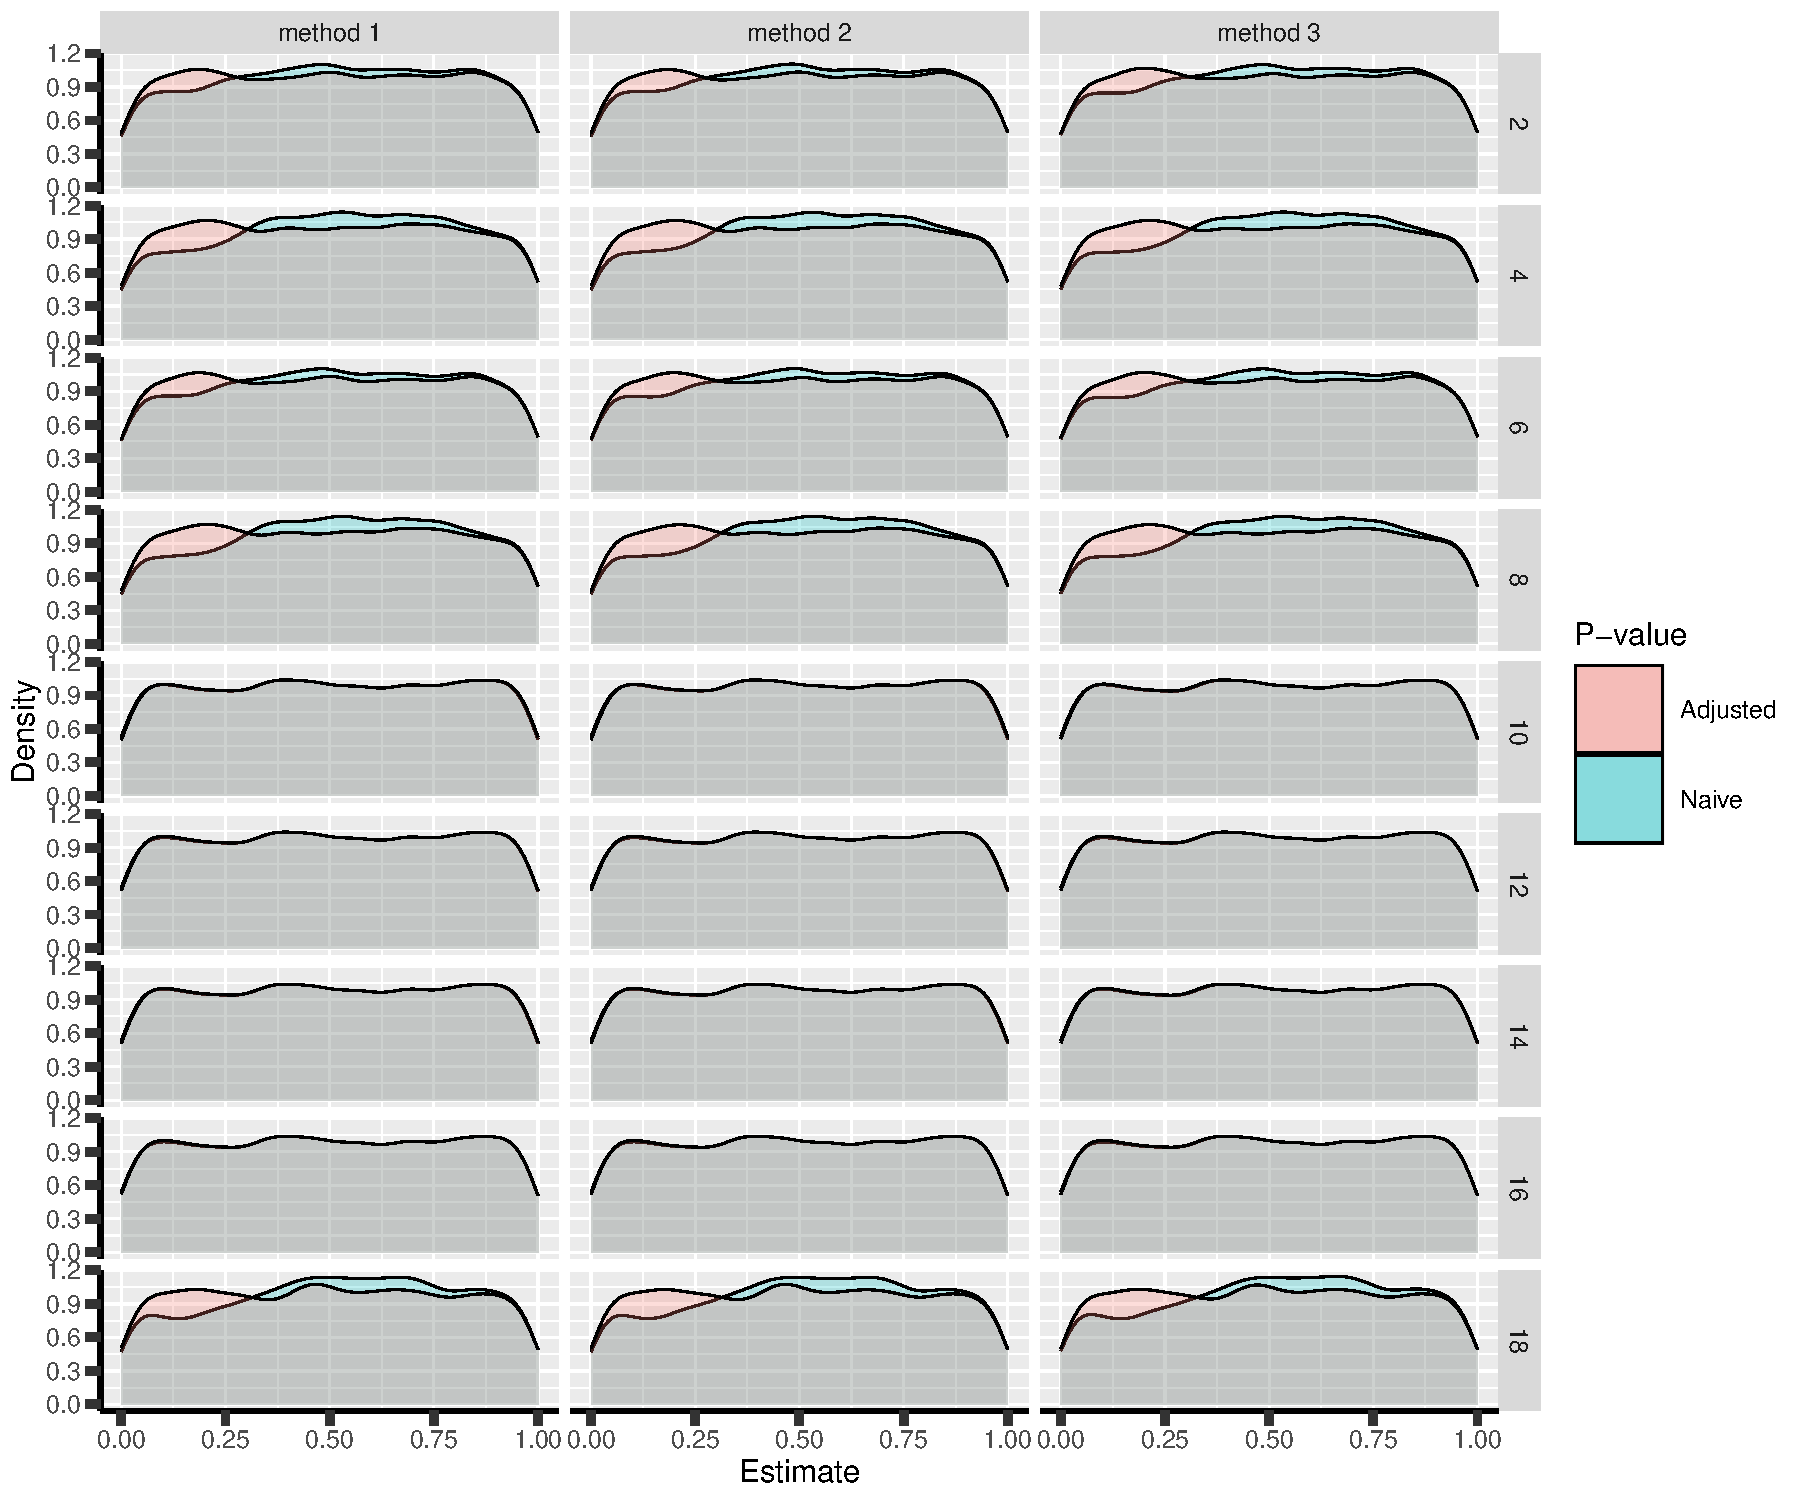
\includegraphics[trim={0 0 0 0},width=1\textwidth]{./figures/gg2stage-pvalue-density.pdf}
\caption{Naive and adjusted p-value distribution over all simulations under the null. Each row correspond to a different scenario}
\end{figure}

\begin{figure}[!h]
\centering
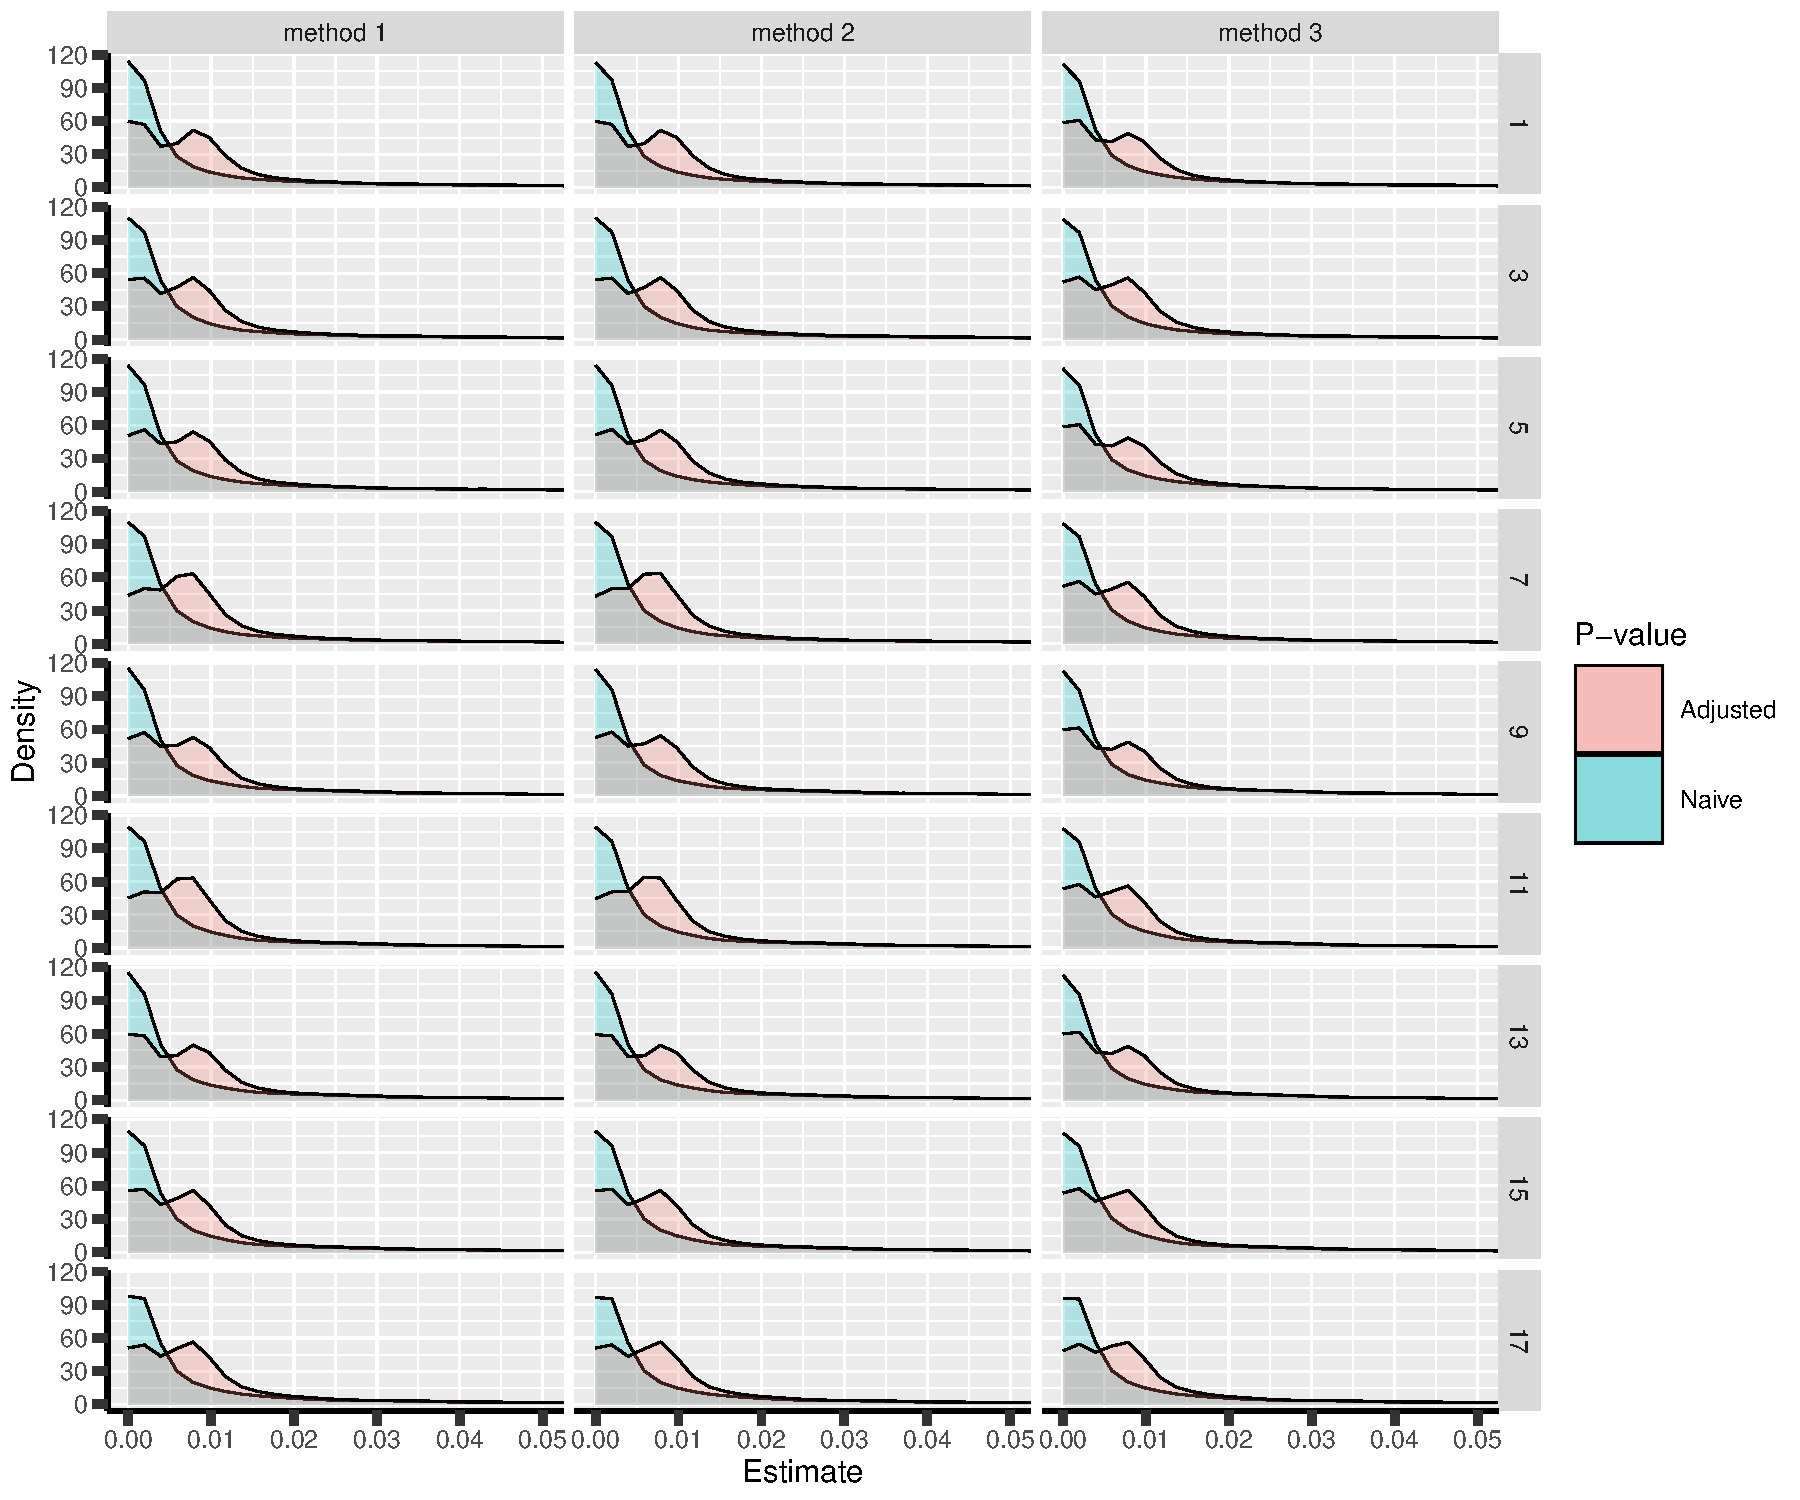
\includegraphics[trim={0 0 0 0},width=1\textwidth]{./figures/gg2stage-pvalue2-density.pdf}
\caption{Naive and adjusted p-value distribution over all simulations under the alternative. Each row correspond to a different scenario}
\end{figure}

\clearpage

\subsection{3 stages}
\label{sec:org726f094}

Power by method (columns) and scenario (rows): \hfill (nominal level 80\%)
\begin{verbatim}
 scenario n.sim missing binding  fixC ar method 1 method 2 method 3
        1 10000    TRUE    TRUE FALSE 10   74.51%   74.51%   74.01%
        3 10000    TRUE    TRUE FALSE  5   74.35%   74.35%   73.99%
        5 10000    TRUE    TRUE  TRUE 10   73.84%   73.91%   74.01%
        7 10000    TRUE    TRUE  TRUE  5   74.00%   74.01%   73.99%
        9 10000    TRUE   FALSE  TRUE 10   74.17%   74.25%   74.45%
       11 10000    TRUE   FALSE  TRUE  5   74.33%   74.37%   74.43%
       13 10000    TRUE   FALSE FALSE 10   74.71%   74.71%   74.45%
       15 10000    TRUE   FALSE FALSE  5   74.61%   74.59%   74.43%
       17 10000   FALSE    TRUE FALSE  5   72.18%   72.18%   71.97%
\end{verbatim}

\bigskip

Type 1 error by method (columns) and scenario (rows): \hfill (nominal level 2.5\%)
\begin{verbatim}
 scenario n.sim missing binding  fixC ar method 1 method 2 method 3
        2 10000    TRUE    TRUE FALSE 10    2.60%    2.60%    2.49%
        4 10000    TRUE    TRUE FALSE  5    2.61%    2.61%    2.59%
        6 10000    TRUE    TRUE  TRUE 10    2.47%    2.50%    2.49%
        8 10000    TRUE    TRUE  TRUE  5    2.56%    2.55%    2.59%
       10  9990    TRUE   FALSE  TRUE 10    2.37%    2.37%    2.42%
       12 10000    TRUE   FALSE  TRUE  5    2.43%    2.44%    2.44%
       14  9990    TRUE   FALSE FALSE 10    2.49%    2.49%    2.42%
       16 10000    TRUE   FALSE FALSE  5    2.53%    2.53%    2.44%
       18 10000   FALSE    TRUE FALSE  5    2.61%    2.61%    2.54%
\end{verbatim}

\clearpage

\begin{figure}[!h]
\centering
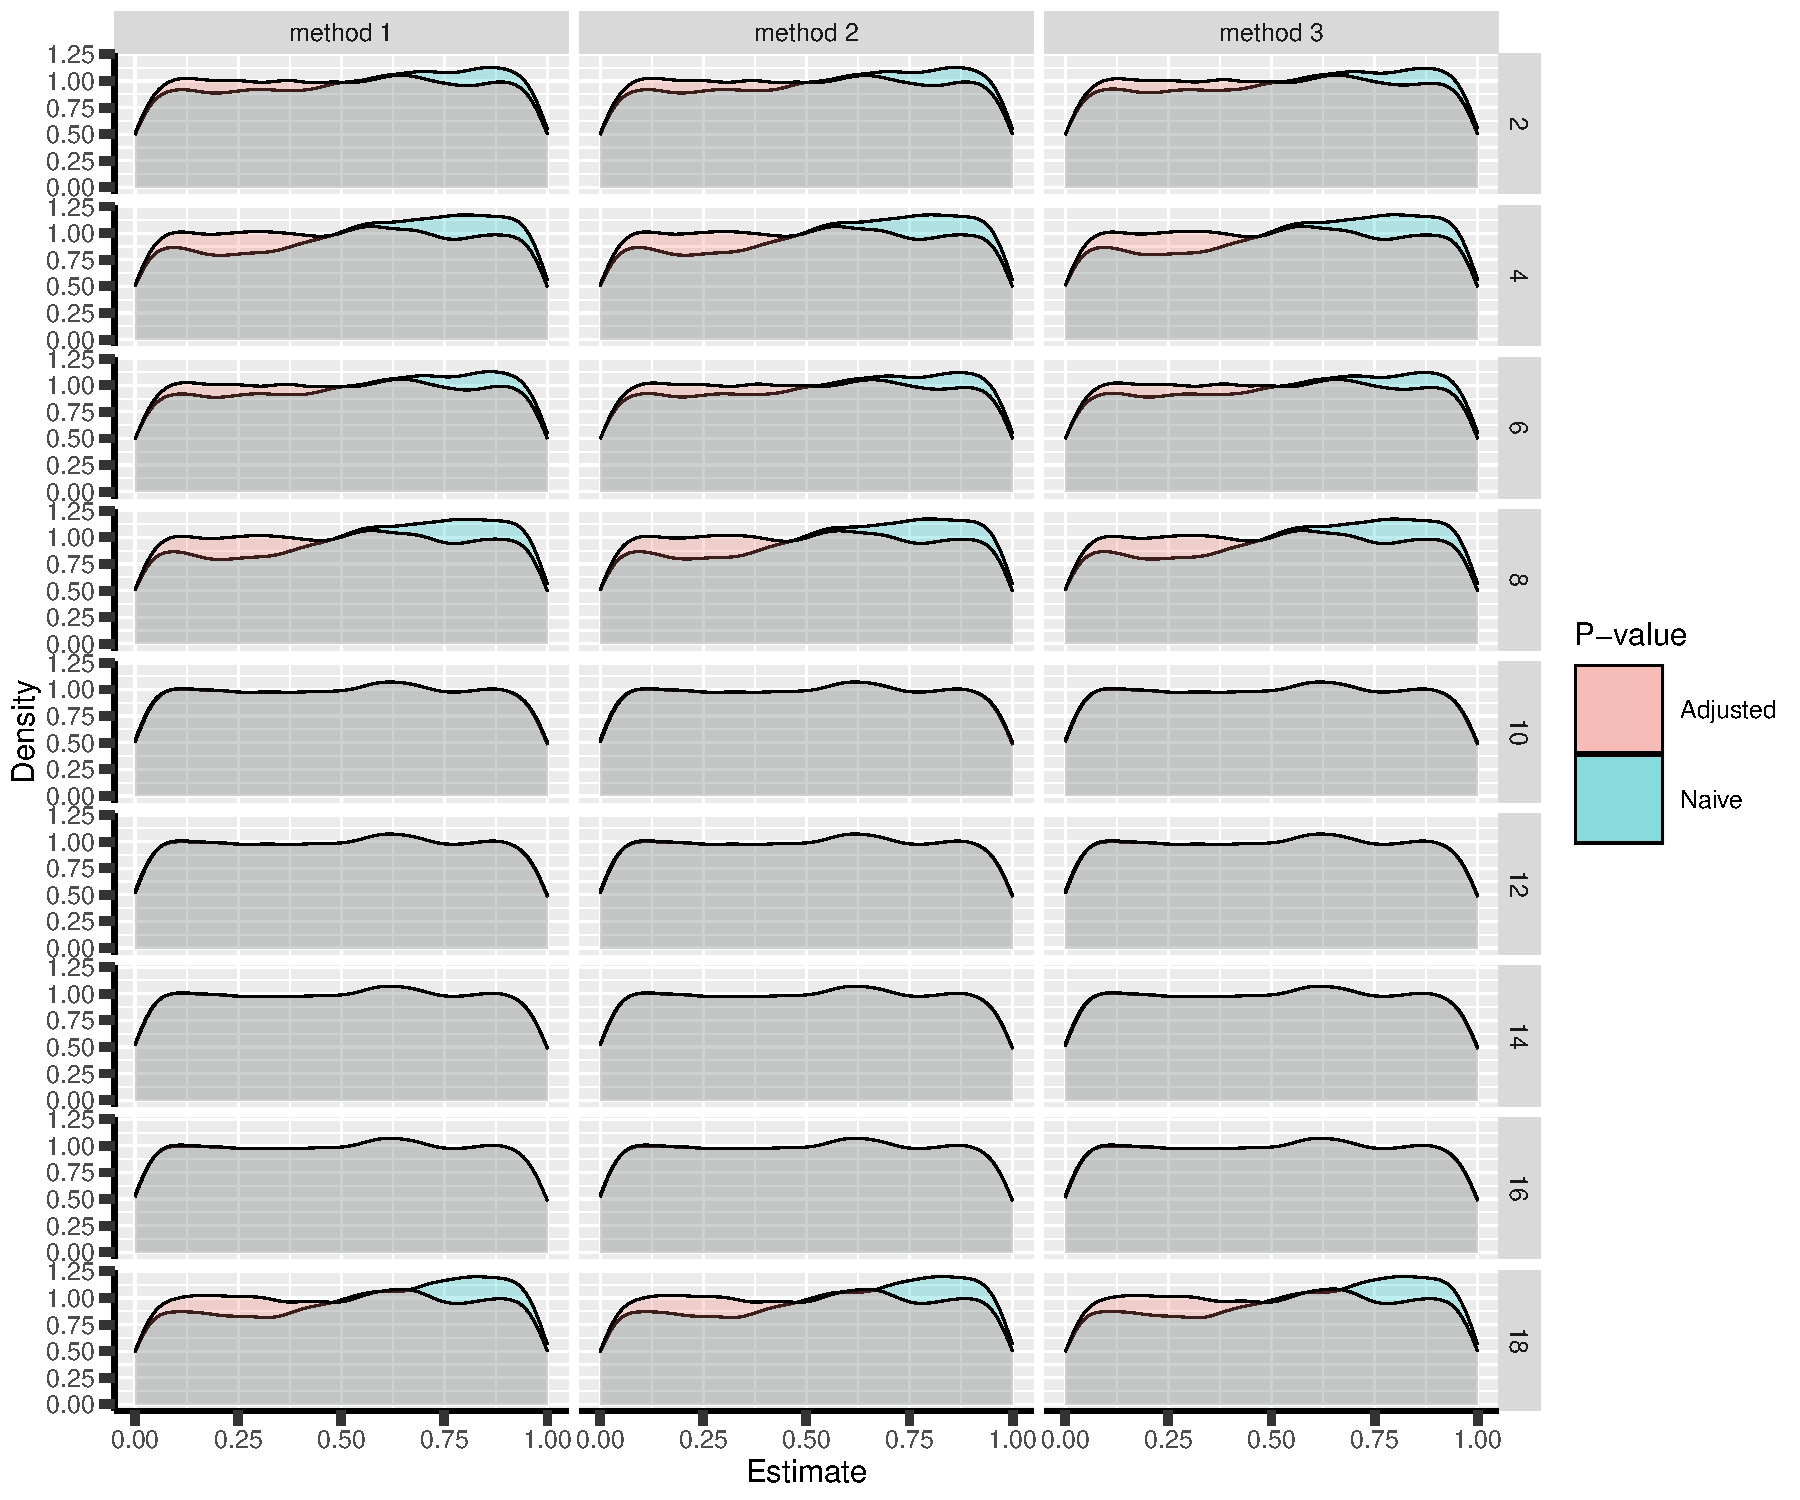
\includegraphics[trim={0 0 0 0},width=1\textwidth]{./figures/gg3stage-pvalue-density.pdf}
\caption{Naive and adjusted p-value distribution over all simulations under the null. Each row correspond to a different scenario}
\end{figure}

\begin{figure}[!h]
\centering
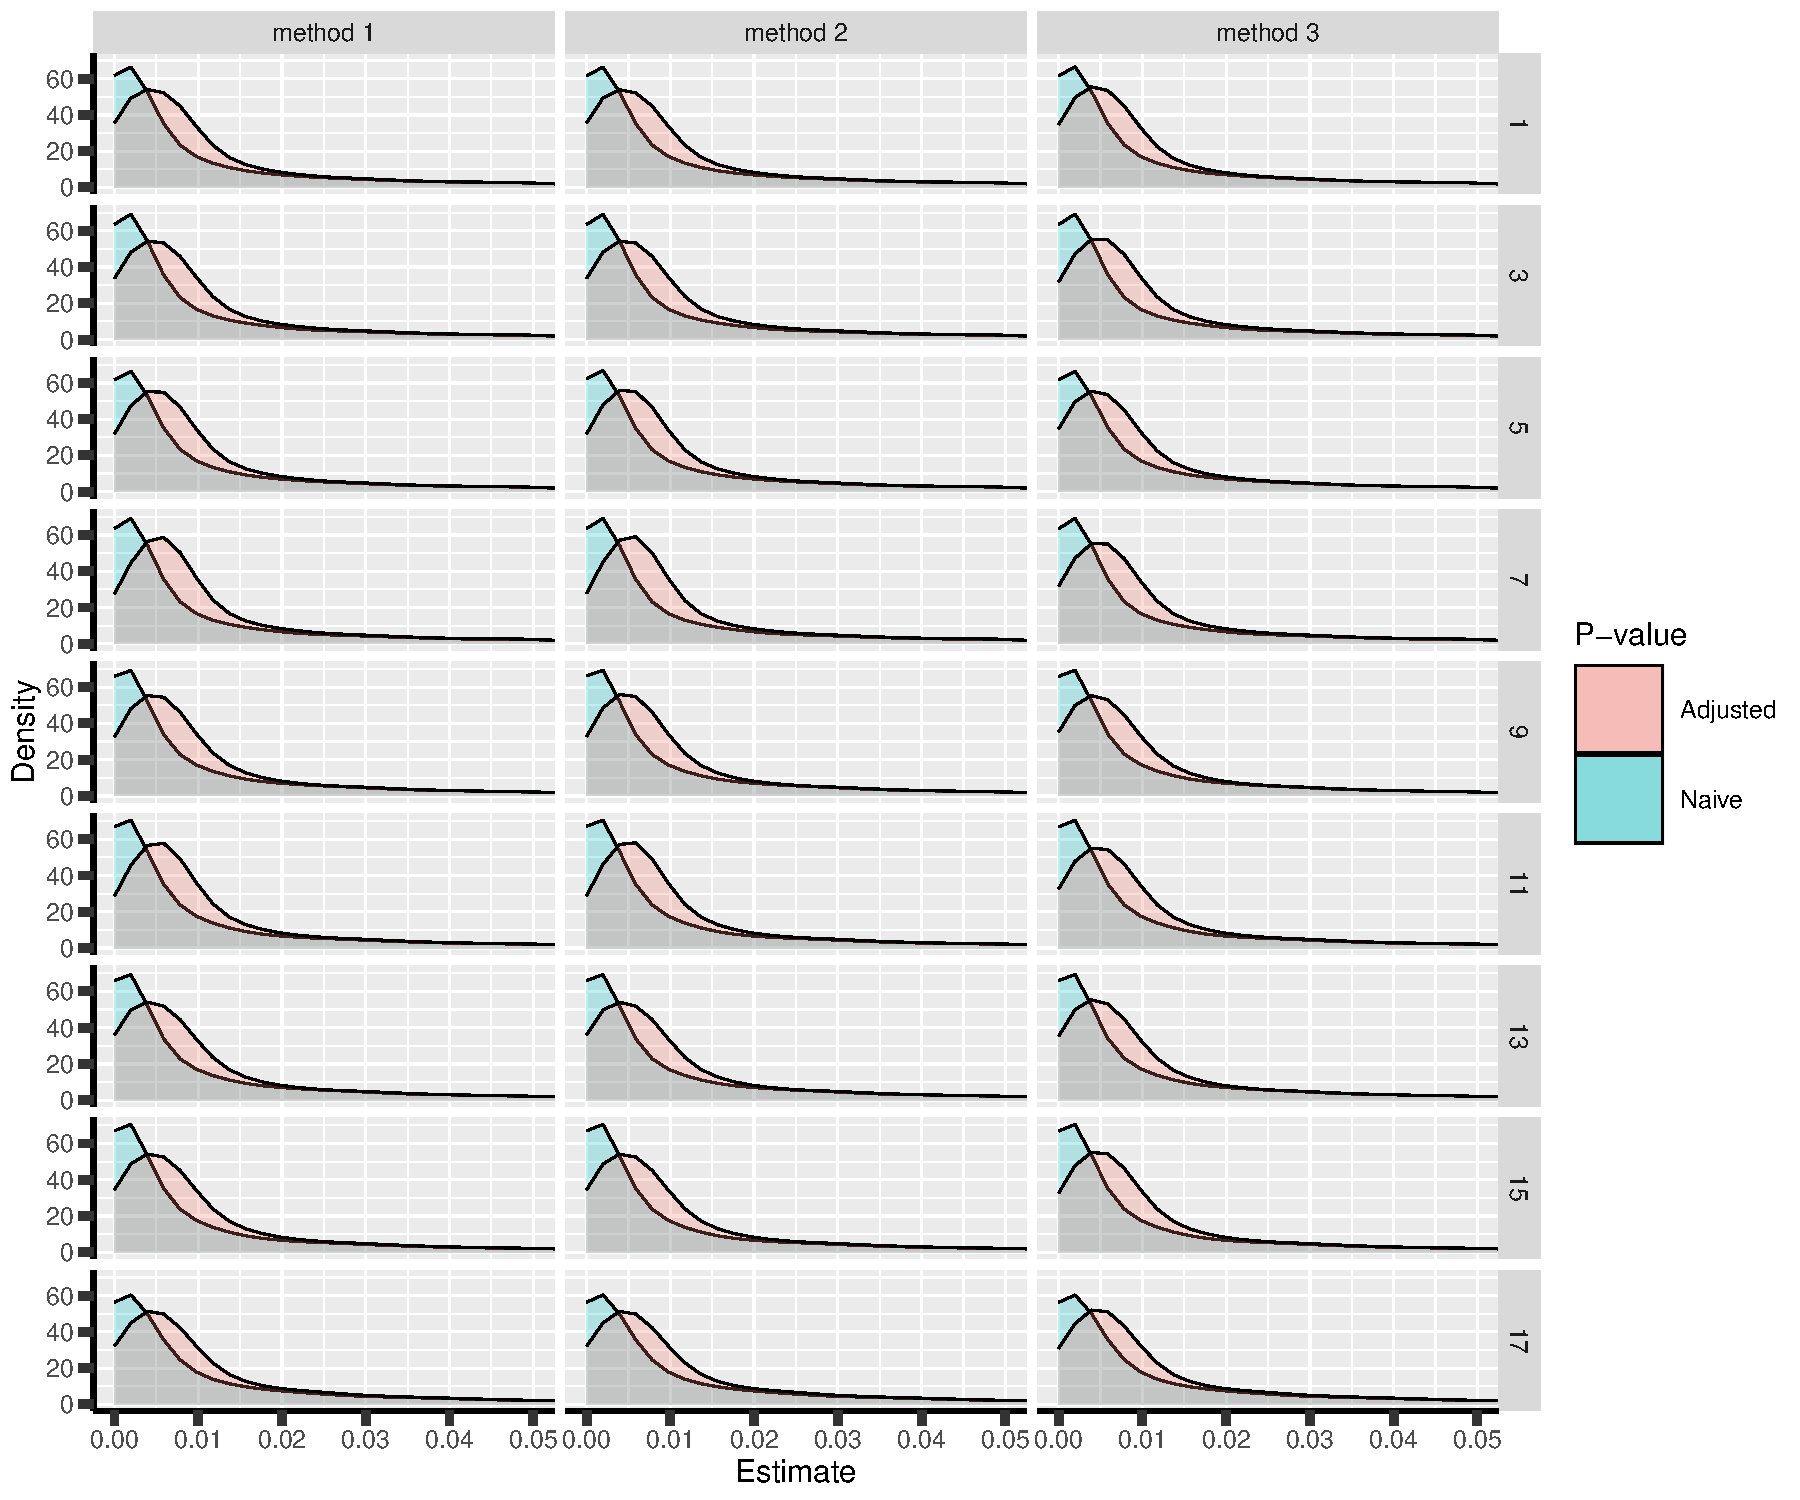
\includegraphics[trim={0 0 0 0},width=1\textwidth]{./figures/gg-pvalue2-density.pdf}
\caption{Naive and adjusted p-value distribution over all simulations under the alternative. Each row correspond to a different scenario}
\end{figure}

\clearpage

\section{Conclusion of the trial}
\label{sec:orga4243b3}

\subsection{2 stages}
\label{sec:org656a578}
Relative frequency of stopping for efficacy/futility at decision/final

\begin{itemize}
\item Method 1
\end{itemize}
\begin{verbatim}
        N missing  hypo binding  fixC ar decision.eff decision.fut final.eff final.fut
 1: 10000    TRUE power    TRUE FALSE 10       37.79%        5.93%    43.21%    13.07%
 2: 10000    TRUE typeI    TRUE FALSE 10        0.80%       71.13%     1.62%    26.45%
 3: 10000    TRUE power    TRUE FALSE  5       35.74%        5.98%    44.79%    13.49%
 4: 10000    TRUE typeI    TRUE FALSE  5        0.74%       69.32%     1.66%    28.28%
 5: 10000    TRUE power    TRUE  TRUE 10       36.94%        6.78%    43.21%    13.07%
 6: 10000    TRUE typeI    TRUE  TRUE 10        0.62%       71.31%     1.62%    26.45%
 7: 10000    TRUE power    TRUE  TRUE  5       35.29%        6.43%    44.79%    13.49%
 8: 10000    TRUE typeI    TRUE  TRUE  5        0.66%       69.40%     1.66%    28.28%
 9: 10000    TRUE power   FALSE  TRUE 10       38.05%        6.57%    41.81%    13.57%
10: 10000    TRUE typeI   FALSE  TRUE 10        0.61%        0.20%     1.84%    97.35%
11: 10000    TRUE power   FALSE  TRUE  5       36.35%        6.15%    43.58%    13.92%
12: 10000    TRUE typeI   FALSE  TRUE  5        0.70%        0.06%     1.93%    97.31%
13: 10000    TRUE power   FALSE FALSE 10       38.69%        5.93%    41.81%    13.57%
14: 10000    TRUE typeI   FALSE FALSE 10        0.69%        0.12%     1.84%    97.35%
15: 10000    TRUE power   FALSE FALSE  5       36.79%        5.71%    43.58%    13.92%
16: 10000    TRUE typeI   FALSE FALSE  5        0.75%        0.01%     1.93%    97.31%
17: 10000   FALSE power    TRUE FALSE  5       33.98%        5.33%    46.33%    14.36%
18: 10000   FALSE typeI    TRUE FALSE  5        0.74%       67.48%     1.72%    30.06%
\end{verbatim}

\clearpage

Method 2:
\begin{verbatim}
        N missing  hypo binding  fixC ar decision.eff decision.fut final.eff final.fut
 1: 10000    TRUE power    TRUE FALSE 10       37.85%        6.19%    43.08%    12.88%
 2: 10000    TRUE typeI    TRUE FALSE 10        0.79%       71.64%     1.60%    25.97%
 3: 10000    TRUE power    TRUE FALSE  5       35.77%        5.99%    44.76%    13.48%
 4: 10000    TRUE typeI    TRUE FALSE  5        0.74%       69.38%     1.66%    28.22%
 5: 10000    TRUE power    TRUE  TRUE 10       36.69%        6.24%    43.66%    13.41%
 6: 10000    TRUE typeI    TRUE  TRUE 10        0.59%       69.61%     1.63%    28.17%
 7: 10000    TRUE power    TRUE  TRUE  5       35.02%        6.05%    45.18%    13.75%
 8: 10000    TRUE typeI    TRUE  TRUE  5        0.63%       68.36%     1.68%    29.33%
 9: 10000    TRUE power   FALSE  TRUE 10       37.85%        6.04%    42.27%    13.84%
10: 10000    TRUE typeI   FALSE  TRUE 10        0.61%        0.19%     1.86%    97.34%
11: 10000    TRUE power   FALSE  TRUE  5       36.18%        5.84%    43.86%    14.12%
12: 10000    TRUE typeI   FALSE  TRUE  5        0.69%        0.06%     1.95%    97.30%
13: 10000    TRUE power   FALSE FALSE 10       38.70%        6.09%    41.74%    13.47%
14: 10000    TRUE typeI   FALSE FALSE 10        0.69%        0.12%     1.84%    97.35%
15: 10000    TRUE power   FALSE FALSE  5       36.82%        5.75%    43.54%    13.89%
16: 10000    TRUE typeI   FALSE FALSE  5        0.75%        0.01%     1.93%    97.31%
17: 10000   FALSE power    TRUE FALSE  5       34.03%        5.36%    46.27%    14.34%
18: 10000   FALSE typeI    TRUE FALSE  5        0.74%       67.55%     1.72%    29.99%
\end{verbatim}

Method 3:
\begin{verbatim}
        N missing  hypo binding  fixC ar decision.eff decision.fut final.eff final.fut
 1: 10000    TRUE power    TRUE FALSE 10       40.58%        6.53%    39.85%    13.04%
 2: 10000    TRUE typeI    TRUE FALSE 10        0.74%       68.79%     1.63%    28.84%
 3: 10000    TRUE power    TRUE FALSE  5       36.54%        6.30%    43.60%    13.56%
 4: 10000    TRUE typeI    TRUE FALSE  5        0.69%       68.41%     1.66%    29.24%
 5: 10000    TRUE power    TRUE  TRUE 10       40.58%        6.53%    39.85%    13.04%
 6: 10000    TRUE typeI    TRUE  TRUE 10        0.74%       68.79%     1.63%    28.84%
 7: 10000    TRUE power    TRUE  TRUE  5       36.54%        6.30%    43.60%    13.56%
 8: 10000    TRUE typeI    TRUE  TRUE  5        0.69%       68.41%     1.66%    29.24%
 9: 10000    TRUE power   FALSE  TRUE 10       41.34%        6.20%    38.92%    13.54%
10: 10000    TRUE typeI   FALSE  TRUE 10        0.77%        0.33%     1.80%    97.10%
11: 10000    TRUE power   FALSE  TRUE  5       37.71%        6.03%    42.35%    13.91%
12: 10000    TRUE typeI   FALSE  TRUE  5        0.73%        0.09%     1.93%    97.25%
13: 10000    TRUE power   FALSE FALSE 10       41.34%        6.20%    38.92%    13.54%
14: 10000    TRUE typeI   FALSE FALSE 10        0.77%        0.33%     1.80%    97.10%
15: 10000    TRUE power   FALSE FALSE  5       37.71%        6.03%    42.35%    13.91%
16: 10000    TRUE typeI   FALSE FALSE  5        0.73%        0.09%     1.93%    97.25%
17: 10000   FALSE power    TRUE FALSE  5       34.65%        5.59%    45.27%    14.49%
18: 10000   FALSE typeI    TRUE FALSE  5        0.68%       66.54%     1.77%    31.01%
\end{verbatim}

\clearpage

Relative frequency of stopping for with a threshold below 1.96:
\begin{verbatim}
    scenario missing method binding  fixC ar  hypo     N rejection rejectionBelow196
 1:        1    TRUE      1    TRUE FALSE 10 power 10000    81.00%             0.85%
 2:        1    TRUE      2    TRUE FALSE 10 power 10000    80.93%             0.84%
 3:        2    TRUE      1    TRUE FALSE 10 typeI 10000     2.42%             0.18%
 4:        2    TRUE      2    TRUE FALSE 10 typeI 10000     2.39%             0.17%
 5:        3    TRUE      1    TRUE FALSE  5 power 10000    80.53%             0.45%
 6:        3    TRUE      2    TRUE FALSE  5 power 10000    80.53%             0.45%
 7:        4    TRUE      1    TRUE FALSE  5 typeI 10000     2.40%             0.08%
 8:        4    TRUE      2    TRUE FALSE  5 typeI 10000     2.40%             0.08%
 9:       13    TRUE      1   FALSE FALSE 10 power 10000    80.50%             0.64%
10:       13    TRUE      2   FALSE FALSE 10 power 10000    80.44%             0.64%
11:       14    TRUE      1   FALSE FALSE 10 typeI 10000     2.53%             0.08%
12:       14    TRUE      2   FALSE FALSE 10 typeI 10000     2.53%             0.08%
13:       15    TRUE      1   FALSE FALSE  5 power 10000    80.37%             0.44%
14:       15    TRUE      2   FALSE FALSE  5 power 10000    80.36%             0.44%
15:       16    TRUE      1   FALSE FALSE  5 typeI 10000     2.68%             0.05%
16:       16    TRUE      2   FALSE FALSE  5 typeI 10000     2.68%             0.05%
17:       17   FALSE      1    TRUE FALSE  5 power 10000    80.31%             0.42%
18:       17   FALSE      2    TRUE FALSE  5 power 10000    80.30%             0.43%
19:       18   FALSE      1    TRUE FALSE  5 typeI 10000     2.46%             0.08%
20:       18   FALSE      2    TRUE FALSE  5 typeI 10000     2.46%             0.08%
\end{verbatim}

\clearpage

\subsection{3 stages}
\label{sec:org747d42b}
Relative frequency of stopping for efficacy/futility at decision/final

\begin{itemize}
\item Method 1
\end{itemize}
\begin{verbatim}
        N missing  hypo binding  fixC ar dec1.eff dec1.fut dec2.eff dec2.fut final.eff final.fut
 1: 10000    TRUE power    TRUE FALSE 10    9.46%    1.46%   20.92%    3.30%    44.13%    20.73%
 2: 10000    TRUE typeI    TRUE FALSE 10    0.23%   26.36%    0.48%   35.88%     1.89%    35.16%
 3: 10000    TRUE power    TRUE FALSE  5    9.90%    1.65%   20.79%    3.54%    43.66%    20.46%
 4: 10000    TRUE typeI    TRUE FALSE  5    0.27%   27.41%    0.39%   35.44%     1.95%    34.54%
 5: 10000    TRUE power    TRUE  TRUE 10    9.27%    1.65%   20.44%    3.78%    44.13%    20.73%
 6: 10000    TRUE typeI    TRUE  TRUE 10    0.17%   26.42%    0.41%   35.95%     1.89%    35.16%
 7: 10000    TRUE power    TRUE  TRUE  5    9.75%    1.80%   20.59%    3.74%    43.66%    20.46%
 8: 10000    TRUE typeI    TRUE  TRUE  5    0.25%   27.43%    0.36%   35.47%     1.95%    34.54%
 9: 10000    TRUE power   FALSE  TRUE 10    9.60%    1.62%   20.44%    3.60%    44.13%    20.61%
10:  9990    TRUE typeI   FALSE  TRUE 10    0.16%    0.07%    0.34%    0.11%     1.87%    97.45%
11: 10000    TRUE power   FALSE  TRUE  5   10.34%    1.78%   20.48%    3.35%    43.51%    20.54%
12: 10000    TRUE typeI   FALSE  TRUE  5    0.27%    0.02%    0.36%    0.08%     1.80%    97.47%
13: 10000    TRUE power   FALSE FALSE 10    9.83%    1.39%   20.75%    3.29%    44.13%    20.61%
14:  9990    TRUE typeI   FALSE FALSE 10    0.21%    0.02%    0.41%    0.04%     1.87%    97.45%
15: 10000    TRUE power   FALSE FALSE  5   10.46%    1.66%   20.64%    3.19%    43.51%    20.54%
16: 10000    TRUE typeI   FALSE FALSE  5    0.29%        0    0.44%        0     1.80%    97.47%
17: 10000   FALSE power    TRUE FALSE  5    8.93%    1.66%   19.60%    2.97%    43.65%    23.19%
18: 10000   FALSE typeI    TRUE FALSE  5    0.23%   25.91%    0.38%   34.48%     2.00%    37.00%
\end{verbatim}

\begin{itemize}
\item Method 2
\end{itemize}
\begin{verbatim}
        N missing  hypo binding  fixC ar dec1.eff dec1.fut dec2.eff dec2.fut final.eff final.fut
 1: 10000    TRUE power    TRUE FALSE 10    9.49%    1.47%   20.92%    3.32%    44.10%    20.70%
 2: 10000    TRUE typeI    TRUE FALSE 10    0.23%   26.43%    0.48%   35.92%     1.89%    35.05%
 3: 10000    TRUE power    TRUE FALSE  5    9.91%    1.65%   20.81%    3.55%    43.63%    20.45%
 4: 10000    TRUE typeI    TRUE FALSE  5    0.27%   27.42%    0.39%   35.46%     1.95%    34.51%
 5: 10000    TRUE power    TRUE  TRUE 10    9.14%    1.51%   20.35%    3.43%    44.42%    21.15%
 6: 10000    TRUE typeI    TRUE  TRUE 10    0.17%   25.29%    0.41%   35.73%     1.92%    36.48%
 7: 10000    TRUE power    TRUE  TRUE  5    9.67%    1.74%   20.46%    3.64%    43.88%    20.61%
 8: 10000    TRUE typeI    TRUE  TRUE  5    0.24%   26.94%    0.35%   35.19%     1.96%    35.32%
 9: 10000    TRUE power   FALSE  TRUE 10    9.56%    1.46%   20.30%    3.39%    44.39%    20.90%
10:  9990    TRUE typeI   FALSE  TRUE 10    0.16%    0.07%    0.34%    0.11%     1.87%    97.45%
11: 10000    TRUE power   FALSE  TRUE  5   10.27%    1.74%   20.29%    3.26%    43.81%    20.63%
12: 10000    TRUE typeI   FALSE  TRUE  5    0.27%    0.02%    0.36%    0.07%     1.81%    97.47%
13: 10000    TRUE power   FALSE FALSE 10    9.84%    1.40%   20.75%    3.29%    44.12%    20.60%
14:  9990    TRUE typeI   FALSE FALSE 10    0.21%    0.02%    0.41%    0.04%     1.87%    97.45%
15: 10000    TRUE power   FALSE FALSE  5   10.47%    1.67%   20.64%    3.19%    43.48%    20.55%
16: 10000    TRUE typeI   FALSE FALSE  5    0.29%        0    0.45%        0     1.79%    97.47%
17: 10000   FALSE power    TRUE FALSE  5    8.93%    1.66%   19.62%    2.98%    43.63%    23.18%
18: 10000   FALSE typeI    TRUE FALSE  5    0.23%   25.96%    0.38%   34.49%     2.00%    36.94%
\end{verbatim}

\clearpage

\begin{itemize}
\item Method 3
\end{itemize}
\begin{verbatim}
        N missing  hypo binding  fixC ar dec1.eff dec1.fut dec2.eff dec2.fut final.eff final.fut
 1: 10000    TRUE power    TRUE FALSE 10    9.90%    1.60%   21.38%    3.57%    42.73%    20.82%
 2: 10000    TRUE typeI    TRUE FALSE 10    0.18%   25.24%    0.42%   35.72%     1.89%    36.55%
 3: 10000    TRUE power    TRUE FALSE  5    9.85%    1.79%   20.78%    3.71%    43.36%    20.51%
 4: 10000    TRUE typeI    TRUE FALSE  5    0.25%   27.11%    0.38%   35.31%     1.96%    34.99%
 5: 10000    TRUE power    TRUE  TRUE 10    9.90%    1.60%   21.38%    3.57%    42.73%    20.82%
 6: 10000    TRUE typeI    TRUE  TRUE 10    0.18%   25.24%    0.42%   35.72%     1.89%    36.55%
 7: 10000    TRUE power    TRUE  TRUE  5    9.85%    1.79%   20.78%    3.71%    43.36%    20.51%
 8: 10000    TRUE typeI    TRUE  TRUE  5    0.25%   27.11%    0.38%   35.31%     1.96%    34.99%
 9: 10000    TRUE power   FALSE  TRUE 10   10.35%    1.54%   21.20%    3.42%    42.90%    20.59%
10:  9990    TRUE typeI   FALSE  TRUE 10    0.17%    0.10%    0.38%    0.12%     1.87%    97.36%
11: 10000    TRUE power   FALSE  TRUE  5   10.60%    1.77%   20.68%    3.32%    43.15%    20.48%
12: 10000    TRUE typeI   FALSE  TRUE  5    0.27%    0.03%    0.39%    0.08%     1.78%    97.45%
13: 10000    TRUE power   FALSE FALSE 10   10.35%    1.54%   21.20%    3.42%    42.90%    20.59%
14:  9990    TRUE typeI   FALSE FALSE 10    0.17%    0.10%    0.38%    0.12%     1.87%    97.36%
15: 10000    TRUE power   FALSE FALSE  5   10.60%    1.77%   20.68%    3.32%    43.15%    20.48%
16: 10000    TRUE typeI   FALSE FALSE  5    0.27%    0.03%    0.39%    0.08%     1.78%    97.45%
17: 10000   FALSE power    TRUE FALSE  5    8.94%    1.77%   19.69%    3.03%    43.34%    23.23%
18: 10000   FALSE typeI    TRUE FALSE  5    0.21%   25.61%    0.33%   34.46%     2.00%    37.39%
\end{verbatim}

Relative frequency of stopping for with a threshold below 1.96:
\begin{verbatim}
    scenario missing method binding  fixC ar  hypo     N rejection rejectionBelow196
 1:        1    TRUE      1    TRUE FALSE 10 power 10000    74.51%             0.67%
 2:        1    TRUE      2    TRUE FALSE 10 power 10000    74.51%             0.67%
 3:        2    TRUE      1    TRUE FALSE 10 typeI 10000     2.60%             0.13%
 4:        2    TRUE      2    TRUE FALSE 10 typeI 10000     2.60%             0.13%
 5:        3    TRUE      1    TRUE FALSE  5 power 10000    74.35%             0.35%
 6:        3    TRUE      2    TRUE FALSE  5 power 10000    74.35%             0.35%
 7:        4    TRUE      1    TRUE FALSE  5 typeI 10000     2.61%             0.05%
 8:        4    TRUE      2    TRUE FALSE  5 typeI 10000     2.61%             0.05%
 9:       13    TRUE      1   FALSE FALSE 10 power 10000    74.71%             0.54%
10:       13    TRUE      2   FALSE FALSE 10 power 10000    74.71%             0.54%
11:       14    TRUE      1   FALSE FALSE 10 typeI  9990     2.49%             0.12%
12:       14    TRUE      2   FALSE FALSE 10 typeI  9990     2.49%             0.12%
13:       15    TRUE      1   FALSE FALSE  5 power 10000    74.61%             0.28%
14:       15    TRUE      2   FALSE FALSE  5 power 10000    74.59%             0.28%
15:       16    TRUE      1   FALSE FALSE  5 typeI 10000     2.53%             0.10%
16:       16    TRUE      2   FALSE FALSE  5 typeI 10000     2.53%             0.10%
17:       17   FALSE      1    TRUE FALSE  5 power 10000    72.18%             0.29%
18:       17   FALSE      2    TRUE FALSE  5 power 10000    72.18%             0.29%
19:       18   FALSE      1    TRUE FALSE  5 typeI 10000     2.61%             0.08%
20:       18   FALSE      2    TRUE FALSE  5 typeI 10000     2.61%             0.08%
\end{verbatim}


\clearpage

\section{Bias (True effect: 0.6 under the alternative)}
\label{sec:org76bd5f1}

\subsection{2 stages}
\label{sec:org4824153}
Bias per estimator and method\footnote{e.g. \texttt{biasMLE1} mixed model
estimator (treatment effect), method 1 (boundaries)}:
\begin{adjustwidth}{-1cm}{-1cm}
\begin{verbatim}
     hypo missing binding  fixC ar biasMLE1 biasMLE2 biasMLE3 biasMUE1 biasMUE2 biasMUE3
 1: power    TRUE    TRUE FALSE 10  0.01345  0.01315  0.01468  0.00598  0.00566 -0.00286
 2: typeI    TRUE    TRUE FALSE 10 -0.01794 -0.01784 -0.01856 -0.00453 -0.00448 -0.00513
 3: power    TRUE    TRUE FALSE  5  0.02257  0.02255  0.02358  0.01044  0.01047  0.00364
 4: typeI    TRUE    TRUE FALSE  5 -0.03034 -0.03031 -0.03065 -0.01186 -0.01182 -0.01244
 5: power    TRUE    TRUE  TRUE 10  0.01345  0.01403  0.01468 -0.01482 -0.01515 -0.00286
 6: typeI    TRUE    TRUE  TRUE 10 -0.01794 -0.01871 -0.01856 -0.00553 -0.00619 -0.00513
 7: power    TRUE    TRUE  TRUE  5  0.02257  0.02309  0.02358 -0.01511 -0.01521  0.00364
 8: typeI    TRUE    TRUE  TRUE  5 -0.03034 -0.03085 -0.03065 -0.01249 -0.01307 -0.01244
 9: power    TRUE   FALSE  TRUE 10  0.01433  0.01490  0.01529  0.01725  0.01500  0.02897
10: typeI    TRUE   FALSE  TRUE 10  0.00019  0.00019  0.00051 -0.00087 -0.00079  0.00073
11: power    TRUE   FALSE  TRUE  5  0.02366  0.02402  0.02438  0.01667  0.01524  0.03653
12: typeI    TRUE   FALSE  TRUE  5  0.00091  0.00085  0.00101  0.00033  0.00027  0.00086
13: power    TRUE   FALSE FALSE 10  0.01433  0.01416  0.01529  0.03552  0.03589  0.02897
14: typeI    TRUE   FALSE FALSE 10  0.00019  0.00019  0.00051 -0.00020 -0.00021  0.00073
15: power    TRUE   FALSE FALSE  5  0.02366  0.02365  0.02438  0.04186  0.04202  0.03653
16: typeI    TRUE   FALSE FALSE  5  0.00091  0.00091  0.00101  0.00087  0.00087  0.00086
17: power   FALSE    TRUE FALSE  5  0.02284  0.02277  0.02381  0.01197  0.01196  0.00412
18: typeI   FALSE    TRUE FALSE  5 -0.02952 -0.02945 -0.02992 -0.01111 -0.01106 -0.01172
\end{verbatim}
\end{adjustwidth}

Median bias \footnote{Relative frequency at which the estimate is greater than the truth minus 0.5} per estimator and method:
\begin{adjustwidth}{-1cm}{-1cm}
\begin{verbatim}
     hypo missing binding  fixC ar mbiasMLE1 mbiasMLE2 mbiasMLE3 mbiasMUE1 mbiasMUE2 mbiasMUE3
 1: power    TRUE    TRUE FALSE 10    0.0261    0.0260    0.0301  -0.00240  -0.00250  -0.00545
 2: typeI    TRUE    TRUE FALSE 10   -0.0173   -0.0170   -0.0202   0.00100   0.00075  -0.00015
 3: power    TRUE    TRUE FALSE  5    0.0405    0.0405    0.0432  -0.00345  -0.00335  -0.00545
 4: typeI    TRUE    TRUE FALSE  5   -0.0330   -0.0329   -0.0345   0.00055   0.00055   0.00065
 5: power    TRUE    TRUE  TRUE 10    0.0261    0.0265    0.0301  -0.01110  -0.01050  -0.00545
 6: typeI    TRUE    TRUE  TRUE 10   -0.0173   -0.0197   -0.0202   0.00100  -0.00065  -0.00015
 7: power    TRUE    TRUE  TRUE  5    0.0405    0.0407    0.0432  -0.00865  -0.00755  -0.00545
 8: typeI    TRUE    TRUE  TRUE  5   -0.0330   -0.0346   -0.0345   0.00055   0.00075   0.00065
 9: power    TRUE   FALSE  TRUE 10    0.0326    0.0332    0.0327   0.02719   0.02475   0.02804
10: typeI    TRUE   FALSE  TRUE 10   -0.0009   -0.0009   -0.0009  -0.00190  -0.00185  -0.00025
11: power    TRUE   FALSE  TRUE  5    0.0462    0.0459    0.0489   0.02568   0.02469   0.02799
12: typeI    TRUE   FALSE  TRUE  5   -0.0009   -0.0010   -0.0009  -0.00130  -0.00140  -0.00015
13: power    TRUE   FALSE FALSE 10    0.0326    0.0324    0.0327   0.03094   0.03184   0.02804
14: typeI    TRUE   FALSE FALSE 10   -0.0009   -0.0009   -0.0009  -0.00150  -0.00140  -0.00025
15: power    TRUE   FALSE FALSE  5    0.0462    0.0464    0.0489   0.02832   0.02865   0.02799
16: typeI    TRUE   FALSE FALSE  5   -0.0009   -0.0009   -0.0009  -0.00105  -0.00105  -0.00015
17: power   FALSE    TRUE FALSE  5    0.0383    0.0383    0.0400  -0.00265  -0.00255  -0.00485
18: typeI   FALSE    TRUE FALSE  5   -0.0329   -0.0327   -0.0353   0.00420   0.00420   0.00330
\end{verbatim}

\end{adjustwidth}

\clearpage

\subsection{3 stages}
\label{sec:orgf5c49ff}
Bias per estimator and method\footnote{e.g. \texttt{biasMLE1} mixed model
estimator (treatment effect), method 1 (boundaries)}:
\begin{adjustwidth}{-1cm}{-1cm}
\begin{verbatim}
     hypo missing binding  fixC ar biasMLE1 biasMLE2 biasMLE3 biasMUE1 biasMUE2 biasMUE3
 1: power    TRUE    TRUE FALSE 10   0.0212   0.0212   0.0228   0.0233   0.0233   0.0136
 2: typeI    TRUE    TRUE FALSE 10  -0.0348  -0.0348  -0.0340  -0.0268  -0.0268  -0.0280
 3: power    TRUE    TRUE FALSE  5   0.0344   0.0344   0.0350   0.0258   0.0258   0.0164
 4: typeI    TRUE    TRUE FALSE  5  -0.0563  -0.0562  -0.0560  -0.0336  -0.0335  -0.0339
 5: power    TRUE    TRUE  TRUE 10   0.0212   0.0214   0.0228   0.0077   0.0080   0.0136
 6: typeI    TRUE    TRUE  TRUE 10  -0.0348  -0.0340  -0.0340  -0.0280  -0.0283  -0.0280
 7: power    TRUE    TRUE  TRUE  5   0.0344   0.0345   0.0350   0.0053   0.0056   0.0164
 8: typeI    TRUE    TRUE  TRUE  5  -0.0563  -0.0562  -0.0560  -0.0341  -0.0344  -0.0339
 9: power    TRUE   FALSE  TRUE 10   0.0209   0.0212   0.0224   0.0375   0.0359   0.0422
10: typeI    TRUE   FALSE  TRUE 10   0.0027   0.0027   0.0028   0.0023   0.0023   0.0029
11: power    TRUE   FALSE  TRUE  5   0.0339   0.0340   0.0347   0.0376   0.0369   0.0494
12: typeI    TRUE   FALSE  TRUE  5   0.0037   0.0037   0.0038   0.0034   0.0035   0.0037
13: power    TRUE   FALSE FALSE 10   0.0209   0.0209   0.0224   0.0505   0.0505   0.0422
14: typeI    TRUE   FALSE FALSE 10   0.0027   0.0027   0.0028   0.0031   0.0031   0.0029
15: power    TRUE   FALSE FALSE  5   0.0339   0.0339   0.0347   0.0572   0.0572   0.0494
16: typeI    TRUE   FALSE FALSE  5   0.0037   0.0038   0.0038   0.0044   0.0044   0.0037
17: power   FALSE    TRUE FALSE  5   0.0303   0.0303   0.0310   0.0235   0.0235   0.0149
18: typeI   FALSE    TRUE FALSE  5  -0.0565  -0.0565  -0.0564  -0.0362  -0.0363  -0.0368
\end{verbatim}
\end{adjustwidth}

Median bias \footnote{Relative frequency at which the estimate is greater than the truth minus 0.5} per estimator and method:
\begin{adjustwidth}{-1cm}{-1cm}
\begin{verbatim}
     hypo missing binding  fixC ar mbiasMLE1 mbiasMLE2 mbiasMLE3 mbiasMUE1 mbiasMUE2 mbiasMUE3
 1: power    TRUE    TRUE FALSE 10    0.0281    0.0281    0.0300    0.0072   0.00700    0.0025
 2: typeI    TRUE    TRUE FALSE 10   -0.0389   -0.0388   -0.0376   -0.0001   0.00020    0.0013
 3: power    TRUE    TRUE FALSE  5    0.0391    0.0390    0.0400    0.0081   0.00800    0.0053
 4: typeI    TRUE    TRUE FALSE  5   -0.0660   -0.0658   -0.0660   -0.0015  -0.00115   -0.0013
 5: power    TRUE    TRUE  TRUE 10    0.0281    0.0280    0.0300    0.0013   0.00185    0.0025
 6: typeI    TRUE    TRUE  TRUE 10   -0.0389   -0.0377   -0.0376   -0.0005   0.00075    0.0011
 7: power    TRUE    TRUE  TRUE  5    0.0391    0.0387    0.0400    0.0050   0.00530    0.0053
 8: typeI    TRUE    TRUE  TRUE  5   -0.0660   -0.0660   -0.0660   -0.0016  -0.00120   -0.0012
 9: power    TRUE   FALSE  TRUE 10    0.0175    0.0173    0.0188    0.0233   0.02086    0.0221
10: typeI    TRUE   FALSE  TRUE 10   -0.0036   -0.0036   -0.0036   -0.0045  -0.00451   -0.0040
11: power    TRUE   FALSE  TRUE  5    0.0275    0.0272    0.0287    0.0241   0.02347    0.0252
12: typeI    TRUE   FALSE  TRUE  5   -0.0035   -0.0035   -0.0035   -0.0039  -0.00385   -0.0037
13: power    TRUE   FALSE FALSE 10    0.0175    0.0174    0.0188    0.0260   0.02586    0.0221
14: typeI    TRUE   FALSE FALSE 10   -0.0036   -0.0036   -0.0036   -0.0040  -0.00401   -0.0039
15: power    TRUE   FALSE FALSE  5    0.0275    0.0275    0.0287    0.0255   0.02554    0.0252
16: typeI    TRUE   FALSE FALSE  5   -0.0035   -0.0035   -0.0035   -0.0034  -0.00350   -0.0039
17: power   FALSE    TRUE FALSE  5    0.0244    0.0245    0.0251    0.0036   0.00360    0.0014
18: typeI   FALSE    TRUE FALSE  5   -0.0634   -0.0632   -0.0630   -0.0041  -0.00425   -0.0037
\end{verbatim}

\end{adjustwidth}

\clearpage

\section{Distribution of the estimates}
\label{sec:org58a4e51}

\subsection{2 stages}
\label{sec:org2fee04d}
Distribution of the estimates:
\begin{figure}[!h]
\centering
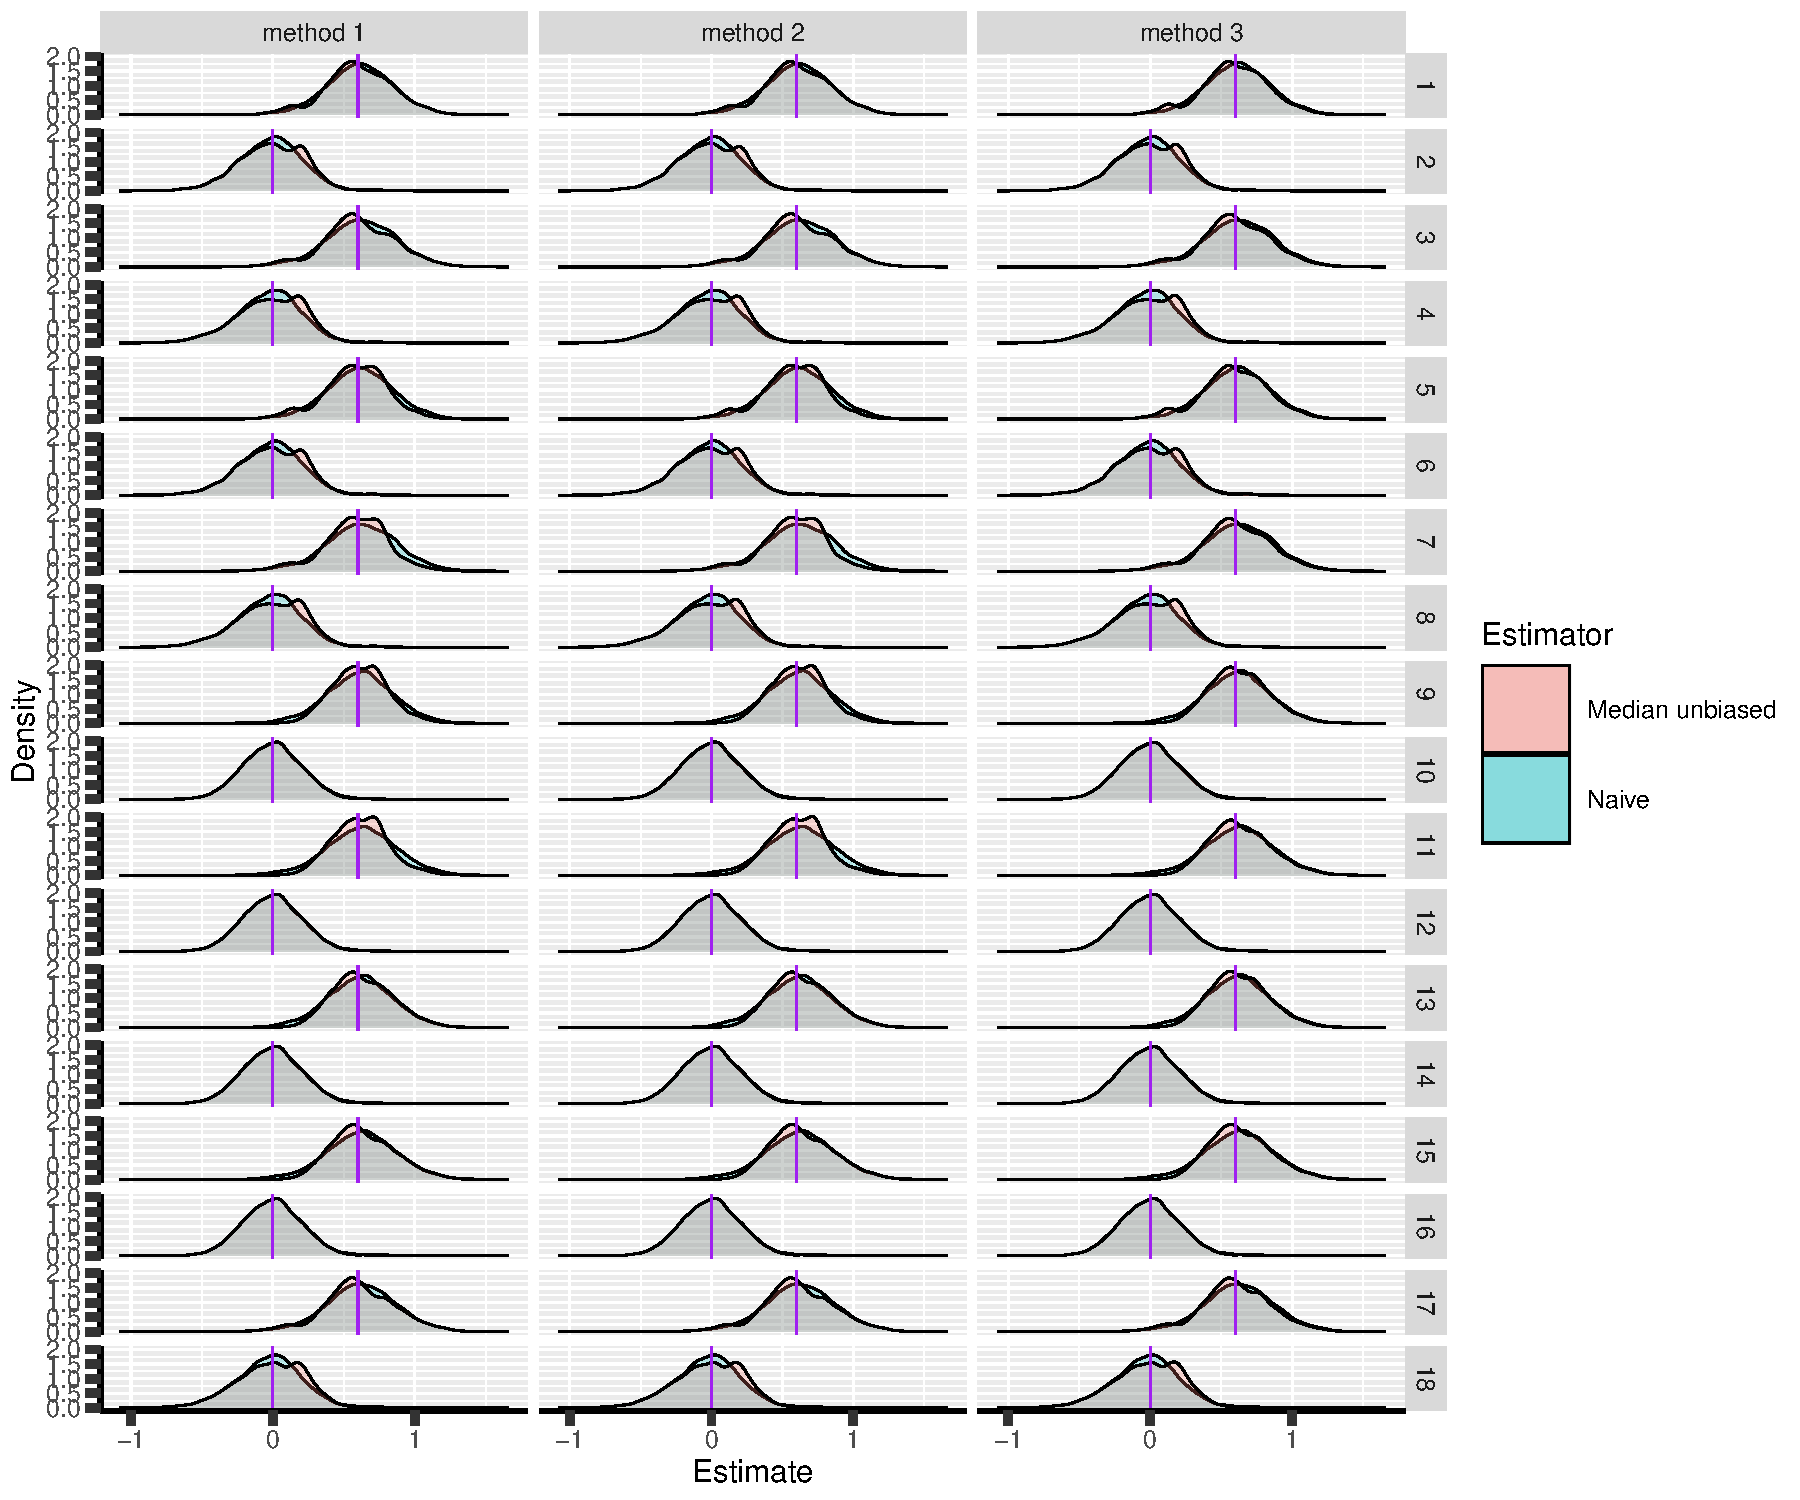
\includegraphics[trim={0 0 0 0},width=1\textwidth]{./figures/gg2stage-estimate-density.pdf}
\caption{Naive and Median unbiased estimate distribution over all simulations. Each row correspond to a different scenario}
\end{figure}

\begin{figure}[!h]
\centering
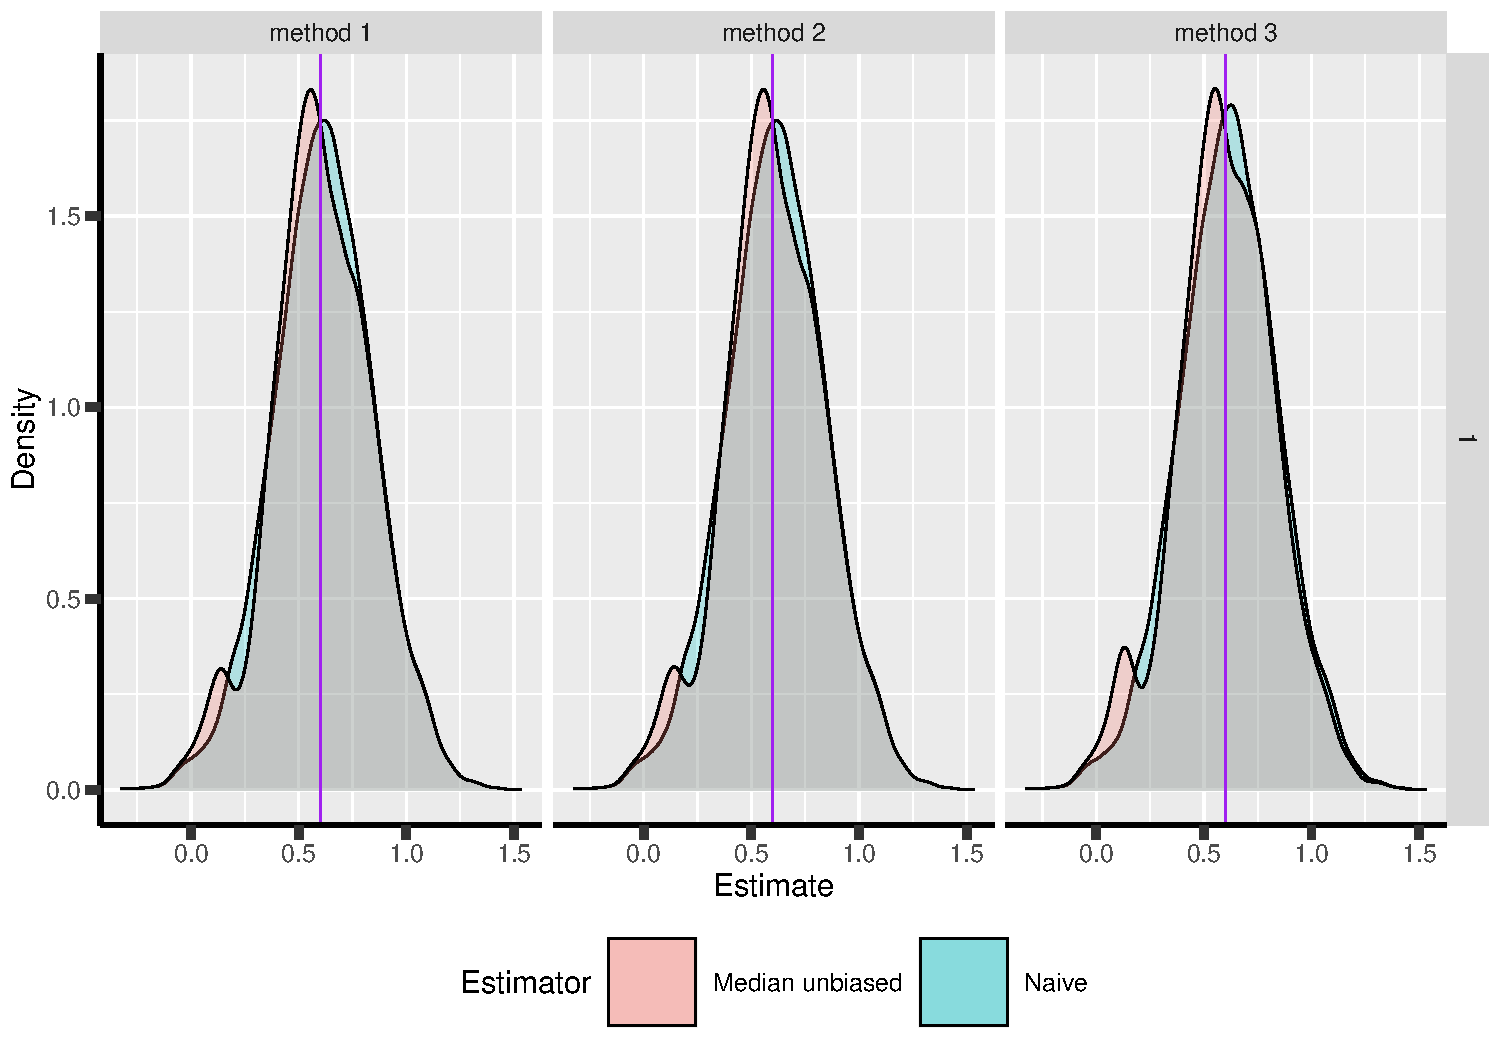
\includegraphics[trim={0 0 0 0},width=\textwidth]{./figures/gg2stage-estimate-density-scenario1.pdf}
\caption{Same but specific to scenario 1}
\end{figure}

\clearpage

Distribution of the median unbiased estimate conditional to the stage:
\begin{figure}[!h]
\centering
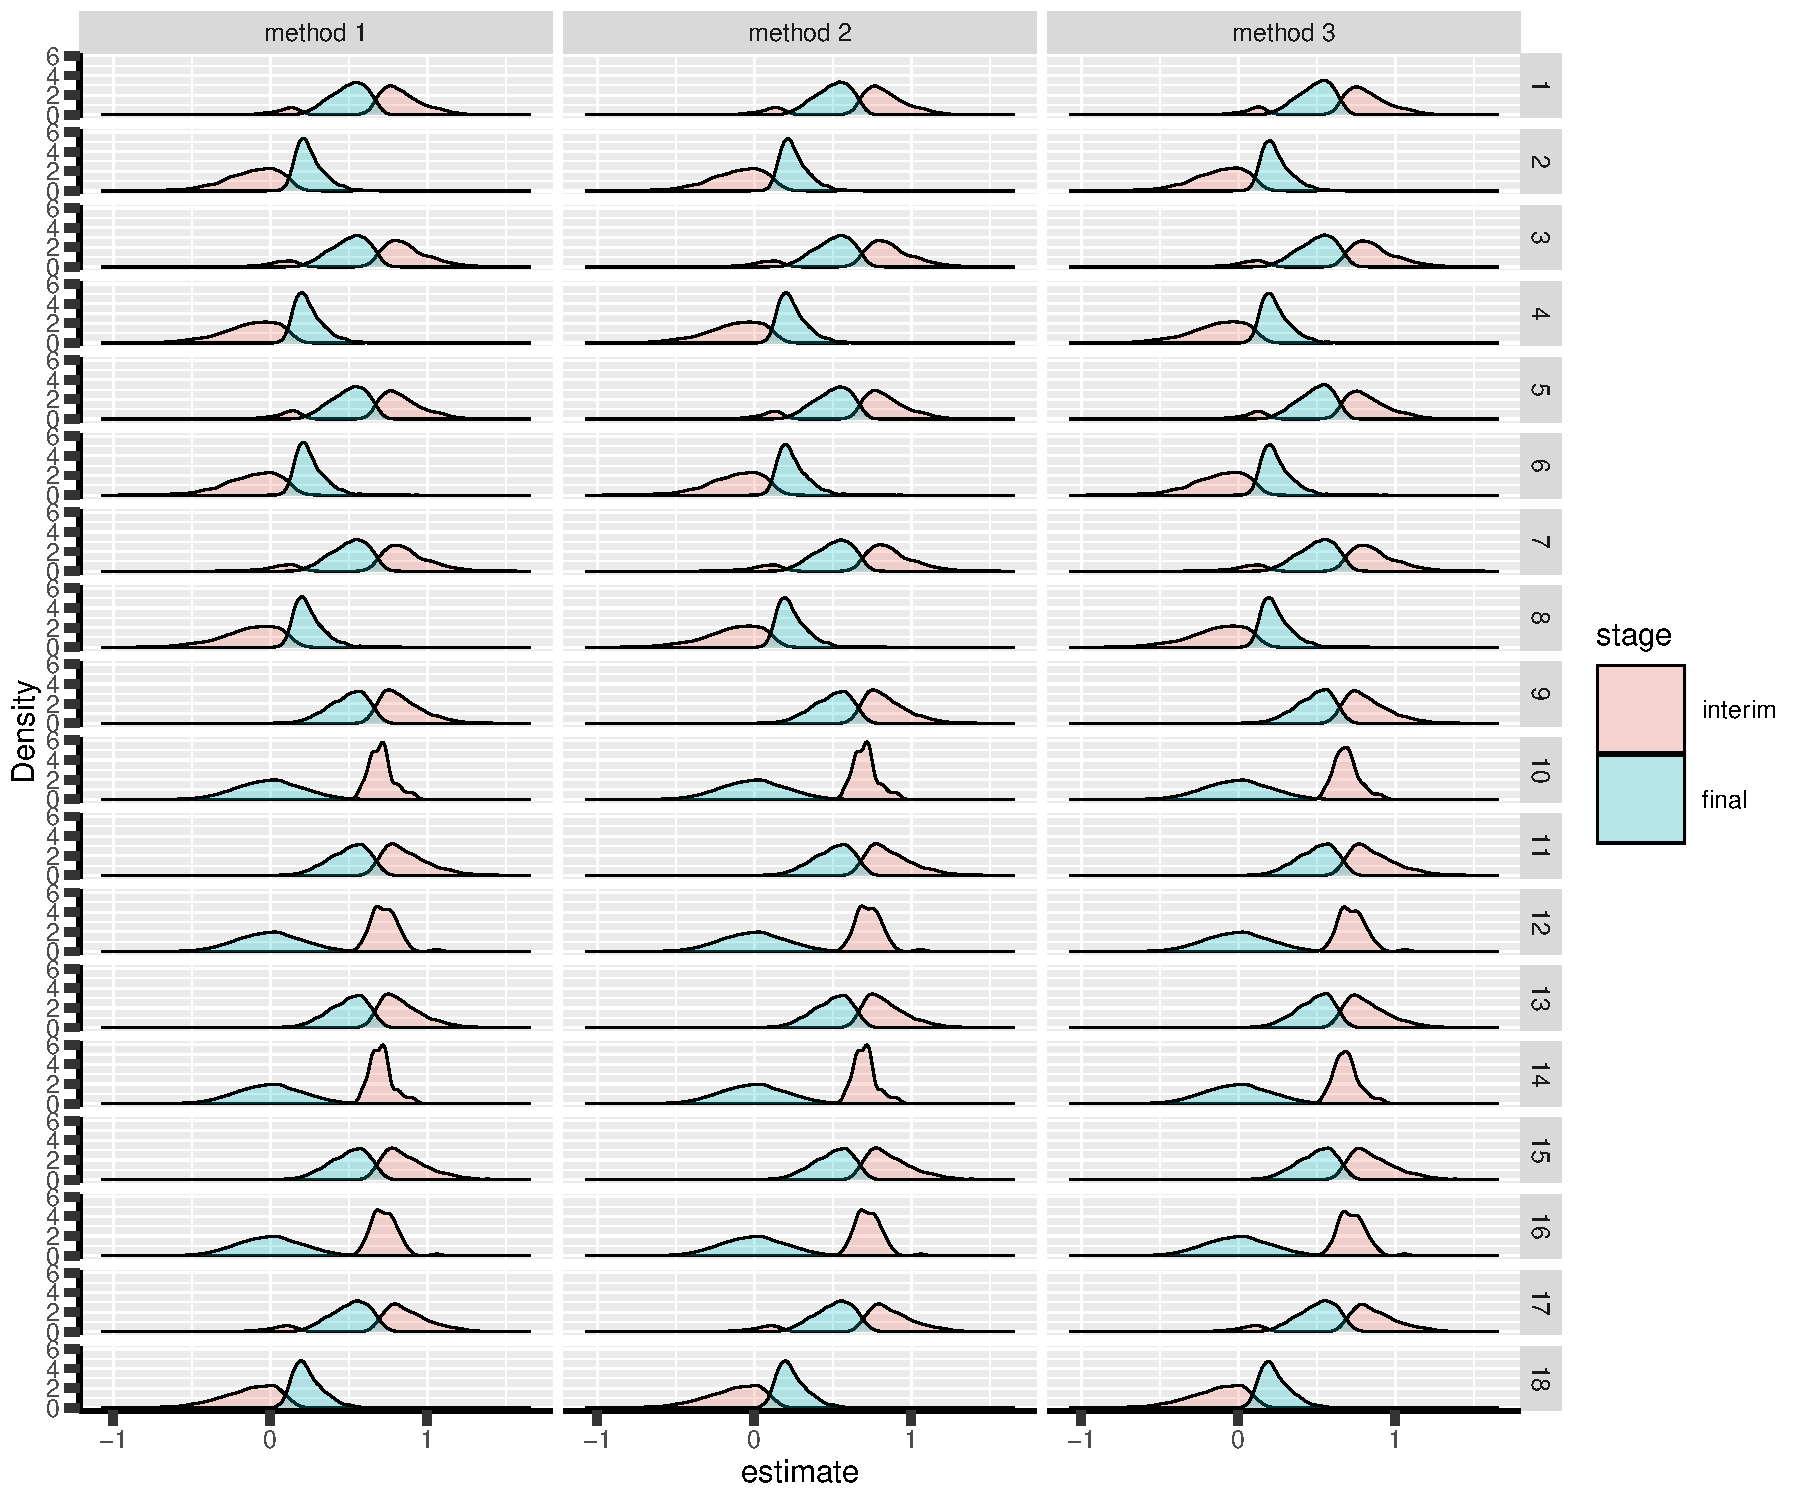
\includegraphics[trim={0 0 0 0},width=1\textwidth]{./figures/gg2stage-estimateC-density.pdf}
\caption{Median unbiased estimate distribution conditional to the stage. Each row correspond to a different scenario.}
\end{figure}

\clearpage

\subsection{3 stages}
\label{sec:orgddcd92f}

Distribution of the estimates:
\begin{figure}[!h]
\centering
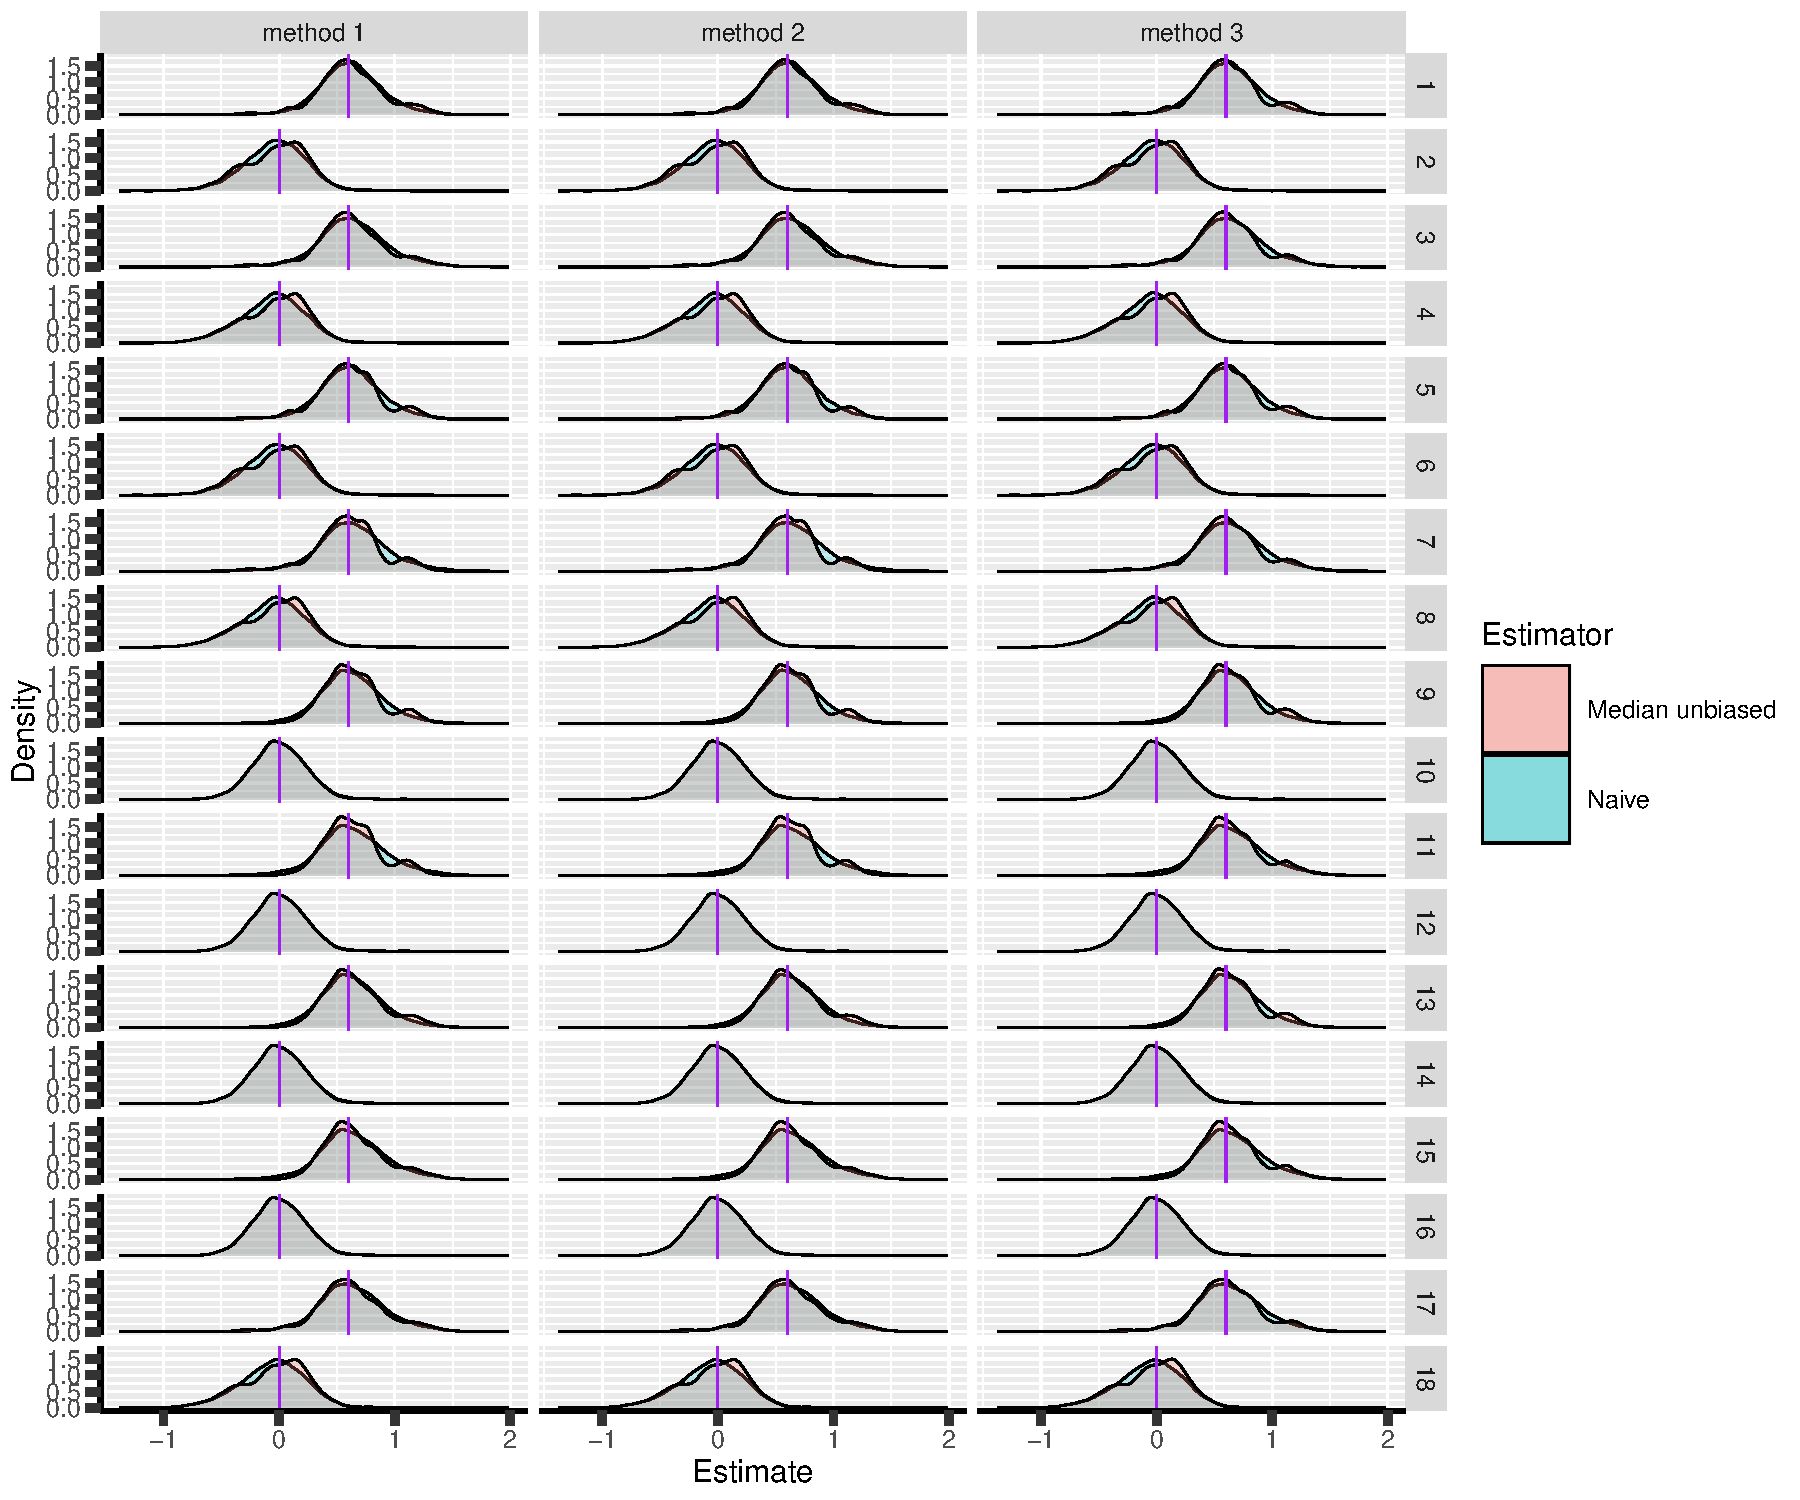
\includegraphics[trim={0 0 0 0},width=1\textwidth]{./figures/gg3stage-estimate-density.pdf}
\caption{Naive and Median unbiased estimate distribution over all simulations. Each row correspond to a different scenario}
\end{figure}

\begin{figure}[!h]
\centering
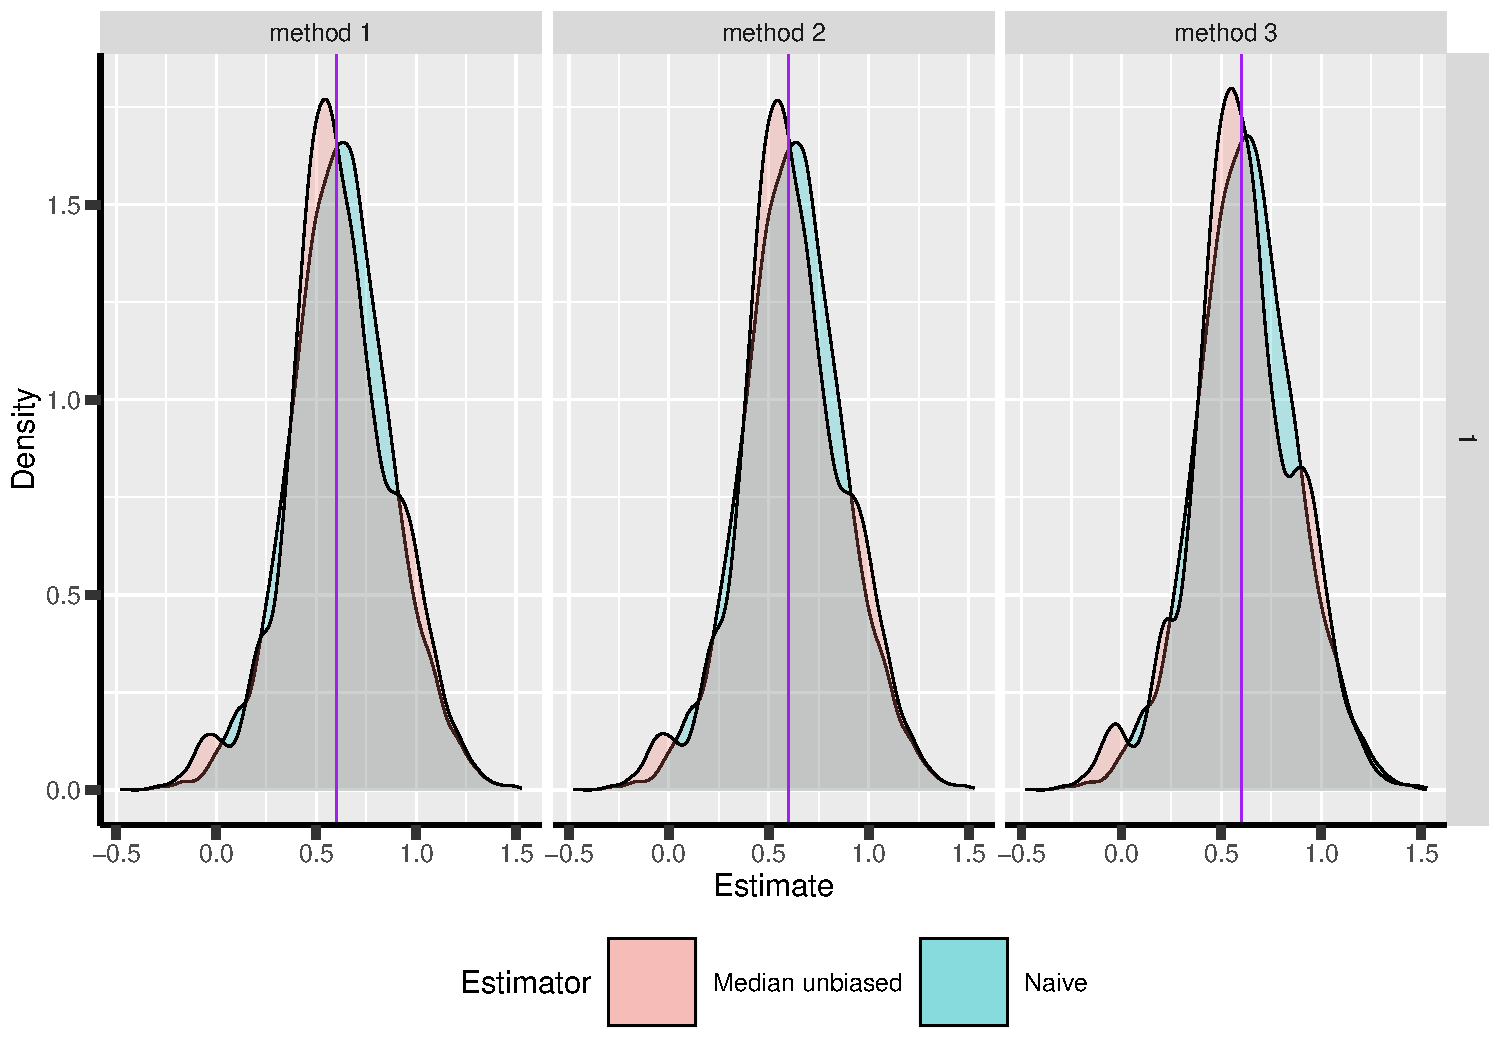
\includegraphics[trim={0 0 0 0},width=\textwidth]{./figures/gg3stage-estimate-density-scenario1.pdf}
\caption{Same but specific to scenario 1}
\end{figure}

\clearpage

Distribution of the median unbiased estimate conditional to the stage:
\begin{figure}[!h]
\centering
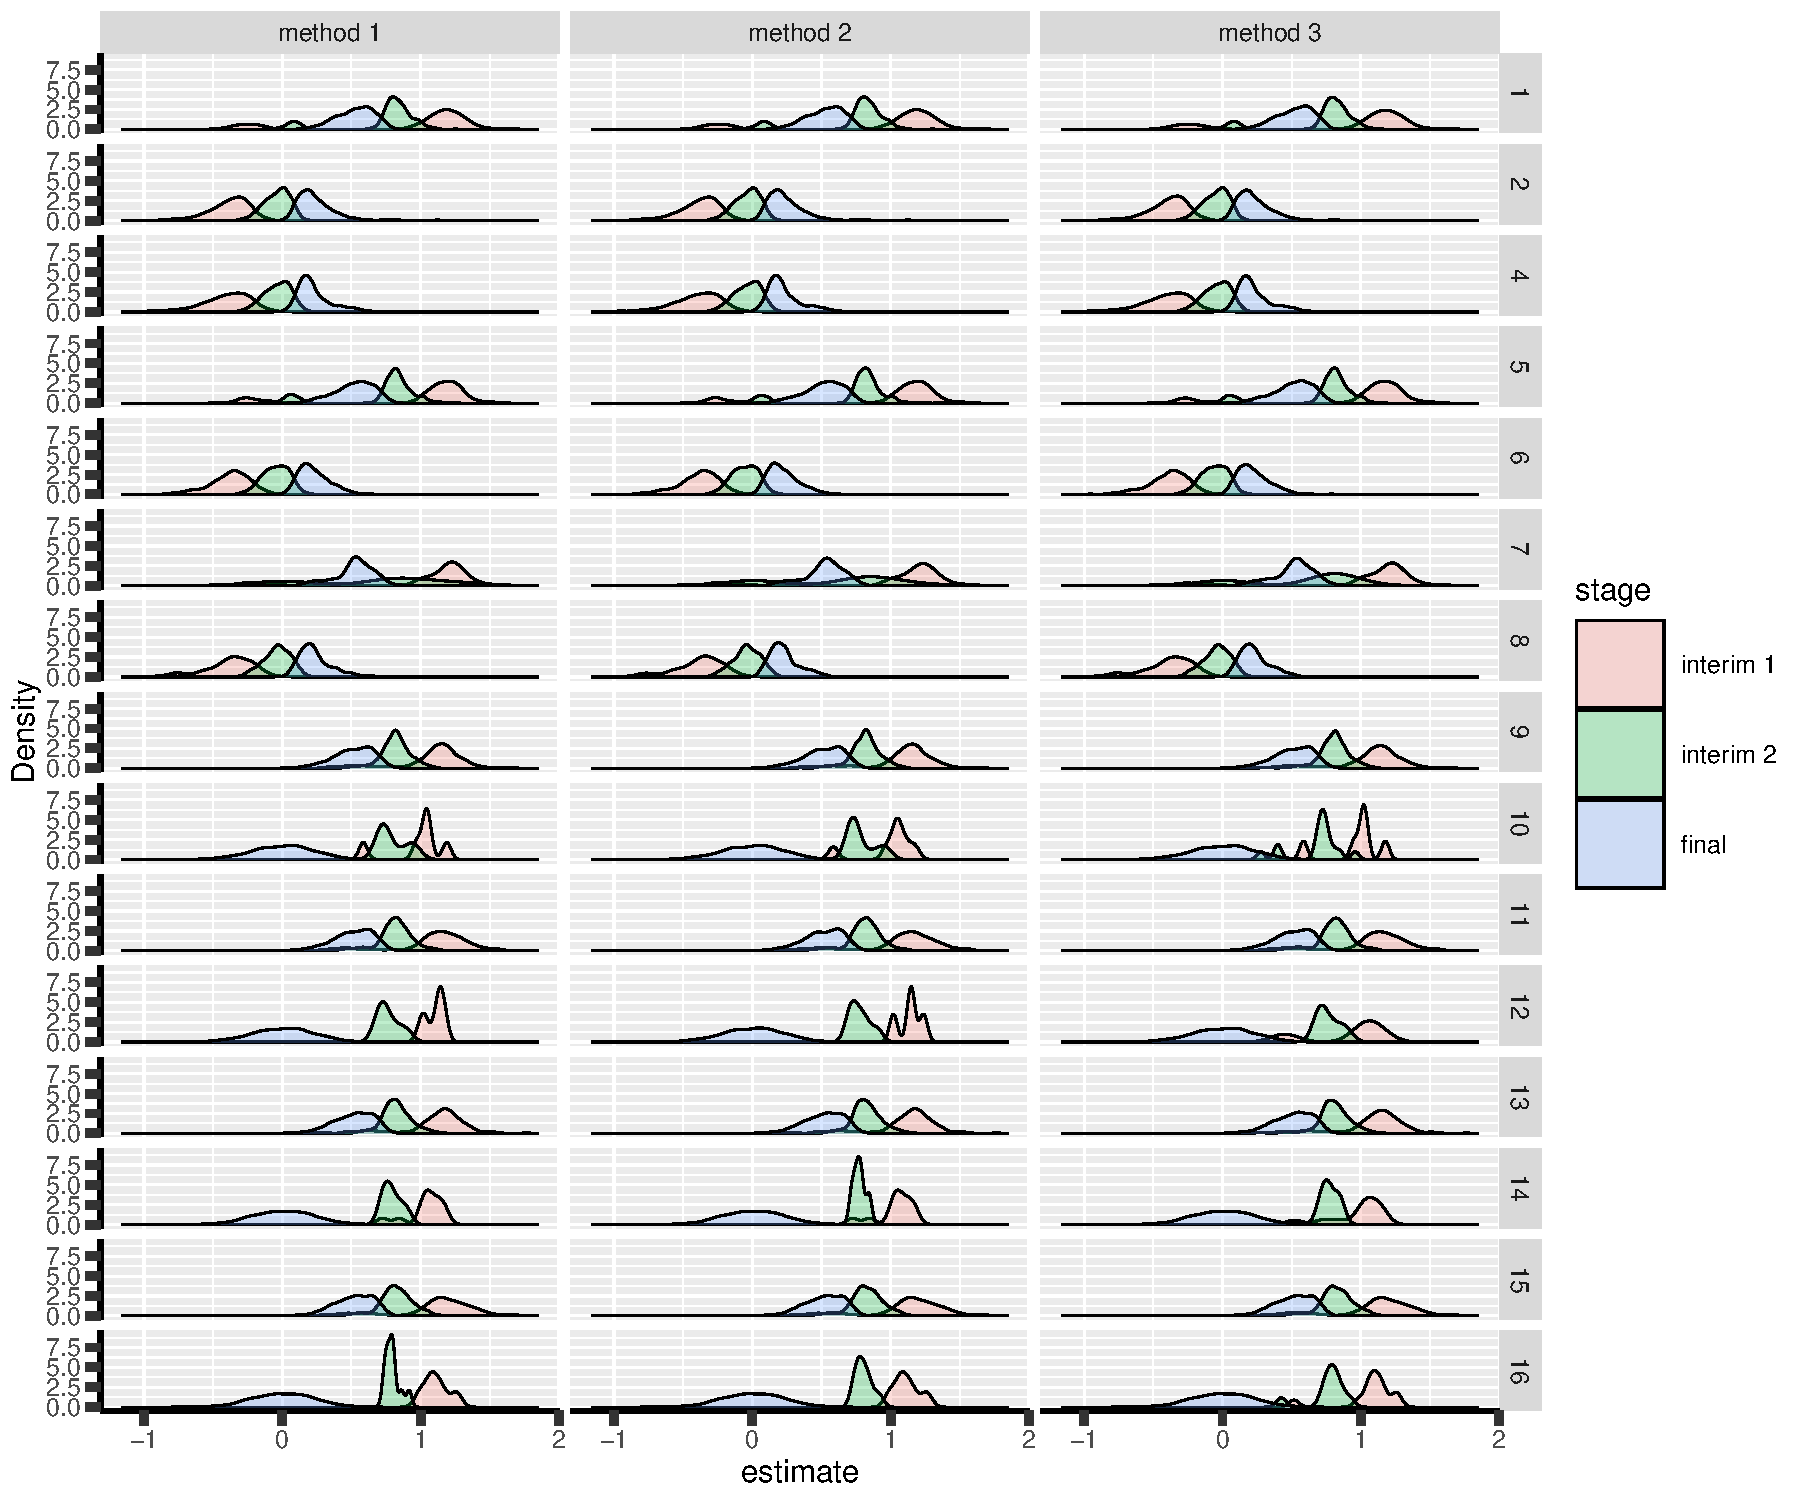
\includegraphics[trim={0 0 0 0},width=1\textwidth]{./figures/gg3stage-estimateC-density.pdf}
\caption{Median unbiased estimate distribution conditional to the stage. Each row correspond to a different scenario.}
\end{figure}

\clearpage

\section{Special cases}
\label{sec:orge48747f}

\subsection{2 stages}
\label{sec:orgdf7099d}

Reason for stopping (efficacy, futility, Imax reached), continuing the
trial (decreasing information, no boundary crossed), or concluding
(stop for futility at interim):
\begin{verbatim}
                                    scenario    1    2    3    4    5    6    7    8
reason                       method                                                 
decreasing information       1                  0    0    1    1    0    0    1    1
                             2                  0    0    1    1    0    0    1    1
                             3                  0    0    1    1    0    0    1    1
efficacy                     1               3739   81 3573   74 3739   81 3573   74
                             2               3744   81 3576   74 3718   79 3545   71
                             3               4165  108 3721   82 4165  108 3721   82
futility                     1                632 7111  599 6932  632 7111  599 6932
                             2                659 7161  600 6938  574 6940  562 6828
                             3                545 6844  563 6828  545 6844  563 6828
Imax reached                 1                  1    1    0    0    1    1    0    0
                             2                  1    1    0    0    1    1    0    0
                             3                  1    1    0    0    1    1    0    0
no boundary crossed          1               5628 2807 5828 2994 5628 2807 5828 2994
                             2               5596 2757 5824 2988 5707 2980 5893 3101
                             3               5289 3047 5716 3090 5289 3047 5716 3090
stop for futility at interim 1                  0    0    0    0    0    0    0    0
                             2                  0    0    0    0    0    0    0    0
                             3                 11    1    2    0   11    1    2    0
\end{verbatim}

\begin{verbatim}
                                    scenario    9   10   11   12   13   14   15   16   17   18
reason                       method                                                           
efficacy                     1               3849   81 3680   76 3849   81 3680   76 3396   74
                             2               3829   80 3661   75 3850   81 3683   76 3400   74
                             3               4238  110 3831   82 4238  110 3831   82 3528   80
futility                     1                613 7122  570 6945  613 7122  570 6945  535 6748
                             2                560 6975  541 6838  629 7164  574 6950  539 6755
                             3                516 6890  543 6842  516 6890  543 6842  496 6642
no boundary crossed          1               5538 2797 5750 2979 5538 2797 5750 2979 6069 3178
                             2               5611 2945 5798 3087 5521 2755 5743 2974 6061 3171
                             3               5246 3000 5626 3076 5246 3000 5626 3076 5976 3278
stop for futility at interim 1                  0    0    0    0    0    0    0    0    0    0
                             2                  0    0    0    0    0    0    0    0    0    0
                             3                  8    0    0    0    8    0    0    0    1    0
\end{verbatim}

\clearpage

\subsection{3 stages}
\label{sec:orga8a1bd4}

Reason for stopping (efficacy, futility, Imax reached), continuing the
trial (decreasing information, no boundary crossed), or concluding
(stop for futility at interim):
\begin{verbatim}
                                    scenario     1     2     3     4     5     6     7     8
reason                       method                                                         
efficacy                     1                3021    71  3070    67  3021    71  3070    67
                             2                3024    71  3073    67  2995    71  3048    65
                             3                3201    82  3108    69  3201    82  3108    69
futility                     1                 493  6224   518  6284   493  6224   518  6284
                             2                 496  6235   519  6287   448  6089   503  6207
                             3                 444  6074   505  6236   444  6074   505  6236
no boundary crossed          1               15394 11046 15257 10881 15394 11046 15257 10881
                             2               15384 11028 15252 10877 15492 11294 15308 11010
                             3               15205 11302 15223 10959 15205 11302 15223 10959
stop for futility at interim 1                   0     0     0     0     0     0     0     0
                             2                   0     0     0     0     0     0     0     0
                             3                   3     1     0     0     3     1     0     0
\end{verbatim}

\begin{verbatim}
                                    scenario     9    10    11    12    13    14    15    16    17    18
reason                       method                                                                     
efficacy                     1                3046    68  3110    73  3046    68  3110    73  2851    61
                             2                3028    68  3083    72  3047    68  3111    74  2853    61
                             3                3212    77  3160    77  3212    77  3160    77  2894    62
futility                     1                 480  8907   485  9058   480  8907   485  9058   465  6039
                             2                 443  8657   473  8953   481  8924   486  9063   466  6045
                             3                 439  8644   477  9002   439  8644   477  9002   449  5999
no boundary crossed          1               15352 10982 15193 10840 15352 10982 15193 10840 15625 11286
                             2               15427 11232 15243 10946 15348 10965 15189 10834 15622 11275
                             3               15160 11232 15126 10891 15160 11232 15126 10891 15586 11357
stop for futility at interim 1                   0     0     0     0     0     0     0     0     0     0
                             2                   0     0     0     0     0     0     0     0     0     0
                             3                   3     0     1     0     3     0     1     0     0     0
\end{verbatim}

\clearpage

\section{Reversal probability}
\label{sec:org02cf1f9}

\subsection{2 stages}
\label{sec:org8549a3a}

Percentage of time we observe a reversal:

\begin{verbatim}
        N  hypo missing ar binding  fixC fu2eff_1 fu2eff_2 fu2eff_3 eff2fu_1 eff2fu_2 eff2fu_3
 1: 10000 power    TRUE 10    TRUE FALSE    0.57%    0.61%        0    0.17%    0.20%    1.07%
 2: 10000 typeI    TRUE 10    TRUE FALSE    0.10%    0.09%        0    0.11%    0.11%    0.34%
 3: 10000 power    TRUE  5    TRUE FALSE    0.08%    0.08%        0    0.07%    0.07%    0.67%
 4: 10000 typeI    TRUE  5    TRUE FALSE    0.02%    0.02%        0    0.02%    0.02%    0.13%
 5: 10000 power    TRUE 10    TRUE  TRUE    0.22%    0.16%        0    0.67%    0.65%    1.07%
 6: 10000 typeI    TRUE 10    TRUE  TRUE    0.02%    0.01%        0    0.21%    0.21%    0.34%
 7: 10000 power    TRUE  5    TRUE  TRUE    0.02%    0.02%        0    0.46%    0.45%    0.67%
 8: 10000 typeI    TRUE  5    TRUE  TRUE        0        0        0    0.08%    0.08%    0.13%
 9: 10000 power    TRUE 10   FALSE  TRUE    0.14%    0.11%        0    0.58%    0.55%    1.04%
10: 10000 typeI    TRUE 10   FALSE  TRUE        0        0        0    0.20%    0.19%    0.33%
11: 10000 power    TRUE  5   FALSE  TRUE    0.01%    0.01%        0    0.46%    0.44%    0.60%
12: 10000 typeI    TRUE  5   FALSE  TRUE        0        0        0    0.06%    0.06%    0.09%
13: 10000 power    TRUE 10   FALSE FALSE    0.41%    0.42%        0    0.21%    0.22%    1.04%
14: 10000 typeI    TRUE 10   FALSE FALSE        0        0        0    0.12%    0.12%    0.33%
15: 10000 power    TRUE  5   FALSE FALSE    0.03%    0.03%        0    0.04%    0.04%    0.60%
16: 10000 typeI    TRUE  5   FALSE FALSE        0        0        0    0.01%    0.01%    0.09%
17: 10000 power   FALSE  5    TRUE FALSE    0.06%    0.07%        0    0.04%    0.04%    0.63%
18: 10000 typeI   FALSE  5    TRUE FALSE    0.01%    0.01%        0    0.01%    0.01%    0.12%
\end{verbatim}

\clearpage

\subsection{3 stages}
\label{sec:org19f7f06}
Percentage of time we observe a reversal:
\begin{verbatim}
        N  hypo missing ar binding  fixC fu2eff_1 fu2eff_2 fu2eff_3 eff2fu_1 eff2fu_2 eff2fu_3
 1: 10000 power    TRUE 10    TRUE FALSE    0.25%    0.25%        0    0.08%    0.08%    0.73%
 2: 10000 typeI    TRUE 10    TRUE FALSE    0.06%    0.06%        0    0.06%    0.06%    0.22%
 3: 10000 typeI    TRUE  5    TRUE FALSE        0        0        0    0.01%    0.01%    0.06%
 4: 10000 power    TRUE 10    TRUE  TRUE    0.04%    0.04%        0    0.54%    0.50%    0.73%
 5: 10000 typeI    TRUE 10    TRUE  TRUE    0.01%    0.01%        0    0.14%    0.14%    0.22%
 6: 10000 power    TRUE  5    TRUE  TRUE        0        0        0    0.36%    0.35%    0.45%
 7: 10000 typeI    TRUE  5    TRUE  TRUE        0        0        0    0.06%    0.06%    0.06%
 8: 10000 power    TRUE 10   FALSE  TRUE    0.05%    0.04%        0    0.47%    0.46%    0.57%
 9:  9990 typeI    TRUE 10   FALSE  TRUE        0        0        0    0.18%    0.18%    0.22%
10: 10000 power    TRUE  5   FALSE  TRUE    0.01%    0.01%        0    0.29%    0.28%    0.32%
11: 10000 typeI    TRUE  5   FALSE  TRUE        0        0        0    0.10%    0.09%    0.11%
12: 10000 power    TRUE 10   FALSE FALSE    0.21%    0.21%        0    0.09%    0.09%    0.57%
13:  9990 typeI    TRUE 10   FALSE FALSE        0        0        0    0.06%    0.06%    0.22%
14: 10000 power    TRUE  5   FALSE FALSE    0.01%    0.01%        0    0.01%    0.01%    0.32%
15: 10000 typeI    TRUE  5   FALSE FALSE        0        0        0        0        0    0.11%
\end{verbatim}


\clearpage

\section{Logical consistency of p-values/CIs}
\label{sec:org1d54d68}

\subsection{Mismatch p-value / boundaries}
\label{sec:orgbcc1256}
\subsubsection{2 stages}
\label{sec:orgf5154bc}

When concluding for futility:
\begin{verbatim}
     hypo missing ar binding  fixC method 1 method 2 method 3
 1: power    TRUE 10    TRUE FALSE        0        0        0
 2: typeI    TRUE 10    TRUE FALSE        0        0        0
 3: power    TRUE  5    TRUE FALSE        0        0        0
 4: typeI    TRUE  5    TRUE FALSE        0        0        0
 5: power    TRUE 10    TRUE  TRUE        0        0        0
 6: typeI    TRUE 10    TRUE  TRUE        0        0        0
 7: power    TRUE  5    TRUE  TRUE        0        0        0
 8: typeI    TRUE  5    TRUE  TRUE        0        0        0
 9: power    TRUE 10   FALSE  TRUE        0        0        0
10: typeI    TRUE 10   FALSE  TRUE        0        0        0
11: power    TRUE  5   FALSE  TRUE        0        0        0
12: typeI    TRUE  5   FALSE  TRUE        0        0        0
13: power    TRUE 10   FALSE FALSE        0        0        0
14: typeI    TRUE 10   FALSE FALSE        0        0        0
15: power    TRUE  5   FALSE FALSE        0        0        0
16: typeI    TRUE  5   FALSE FALSE        0        0        0
17: power   FALSE  5    TRUE FALSE        0        0        0
18: typeI   FALSE  5    TRUE FALSE        0        0        0
\end{verbatim}

When concluding for efficacy:
\begin{verbatim}
     hypo missing ar binding  fixC method 1 method 2 method 3
 1: power    TRUE 10    TRUE FALSE        0        0        0
 2: typeI    TRUE 10    TRUE FALSE        0        0        0
 3: power    TRUE  5    TRUE FALSE        0        0        0
 4: typeI    TRUE  5    TRUE FALSE        0        0        0
 5: power    TRUE 10    TRUE  TRUE        0        0        0
 6: typeI    TRUE 10    TRUE  TRUE        0        0        0
 7: power    TRUE  5    TRUE  TRUE        0        0        0
 8: typeI    TRUE  5    TRUE  TRUE        0        0        0
 9: power    TRUE 10   FALSE  TRUE        0        0        0
10: typeI    TRUE 10   FALSE  TRUE        0        0        0
11: power    TRUE  5   FALSE  TRUE        0        0        0
12: typeI    TRUE  5   FALSE  TRUE        0        0        0
13: power    TRUE 10   FALSE FALSE        0        0        0
14: typeI    TRUE 10   FALSE FALSE        0        0        0
15: power    TRUE  5   FALSE FALSE        0        0        0
16: typeI    TRUE  5   FALSE FALSE        0        0        0
17: power   FALSE  5    TRUE FALSE        0        0        0
18: typeI   FALSE  5    TRUE FALSE        0        0        0
\end{verbatim}

\clearpage

\subsubsection{3 stages}
\label{sec:org1746b3f}

When concluding for futility:
\begin{verbatim}
     hypo missing ar binding  fixC method 1 method 2 method 3
 1: power    TRUE 10    TRUE FALSE        0        0        0
 2: typeI    TRUE 10    TRUE FALSE        0        0        0
 3: power    TRUE  5    TRUE FALSE        0        0        0
 4: typeI    TRUE  5    TRUE FALSE        0        0        0
 5: power    TRUE 10    TRUE  TRUE        0        0    0.04%
 6: typeI    TRUE 10    TRUE  TRUE        0        0        0
 7: power    TRUE  5    TRUE  TRUE        0        0        0
 8: typeI    TRUE  5    TRUE  TRUE        0        0        0
 9: power    TRUE 10   FALSE  TRUE    0.04%    0.04%        0
10: typeI    TRUE 10   FALSE  TRUE        0        0        0
11: power    TRUE  5   FALSE  TRUE        0        0        0
12: typeI    TRUE  5   FALSE  TRUE        0        0        0
13: power    TRUE 10   FALSE FALSE    0.04%        0        0
14: typeI    TRUE 10   FALSE FALSE        0        0        0
15: power    TRUE  5   FALSE FALSE        0        0        0
16: typeI    TRUE  5   FALSE FALSE        0        0        0
17: power   FALSE  5    TRUE FALSE        0        0        0
18: typeI   FALSE  5    TRUE FALSE        0        0        0
\end{verbatim}

When concluding for efficacy:
\begin{verbatim}
     hypo missing ar binding  fixC method 1 method 2 method 3
 1: power    TRUE 10    TRUE FALSE    0.01%    0.01%        0
 2: typeI    TRUE 10    TRUE FALSE    0.38%        0        0
 3: power    TRUE  5    TRUE FALSE        0        0        0
 4: typeI    TRUE  5    TRUE FALSE        0        0        0
 5: power    TRUE 10    TRUE  TRUE    0.01%        0        0
 6: typeI    TRUE 10    TRUE  TRUE    0.40%        0        0
 7: power    TRUE  5    TRUE  TRUE        0        0        0
 8: typeI    TRUE  5    TRUE  TRUE        0        0        0
 9: power    TRUE 10   FALSE  TRUE        0        0        0
10: typeI    TRUE 10   FALSE  TRUE        0        0        0
11: power    TRUE  5   FALSE  TRUE    0.01%    0.01%        0
12: typeI    TRUE  5   FALSE  TRUE        0        0        0
13: power    TRUE 10   FALSE FALSE        0    0.01%        0
14: typeI    TRUE 10   FALSE FALSE        0        0        0
15: power    TRUE  5   FALSE FALSE    0.01%        0        0
16: typeI    TRUE  5   FALSE FALSE        0        0        0
17: power   FALSE  5    TRUE FALSE        0        0        0
18: typeI   FALSE  5    TRUE FALSE        0        0        0
\end{verbatim}

\clearpage

\subsection{Mismatch confidence intervals / boundaries}
\label{sec:org4bb3d0c}

\subsubsection{2 stages}
\label{sec:org60347dc}

When concluding for futility:
\begin{verbatim}
     hypo missing ar binding  fixC       method 1       method 2       method 3
 1: power    TRUE 10    TRUE FALSE              0              0  0 (NA: 0.05%)
 2: typeI    TRUE 10    TRUE FALSE              0              0              0
 3: power    TRUE  5    TRUE FALSE              0              0              0
 4: typeI    TRUE  5    TRUE FALSE              0              0              0
 5: power    TRUE 10    TRUE  TRUE              0              0  0 (NA: 0.05%)
 6: typeI    TRUE 10    TRUE  TRUE              0              0              0
 7: power    TRUE  5    TRUE  TRUE              0              0              0
 8: typeI    TRUE  5    TRUE  TRUE              0              0              0
 9: power    TRUE 10   FALSE  TRUE 0 (NA: 32.62%) 0 (NA: 30.38%) 0 (NA: 31.41%)
10: typeI    TRUE 10   FALSE  TRUE  0 (NA: 0.21%)  0 (NA: 0.19%)  0 (NA: 0.34%)
11: power    TRUE  5   FALSE  TRUE 0 (NA: 30.64%) 0 (NA: 29.26%) 0 (NA: 30.24%)
12: typeI    TRUE  5   FALSE  TRUE  0 (NA: 0.06%)  0 (NA: 0.06%)  0 (NA: 0.09%)
13: power    TRUE 10   FALSE FALSE 0 (NA: 30.41%) 0 (NA: 31.13%) 0 (NA: 31.41%)
14: typeI    TRUE 10   FALSE FALSE  0 (NA: 0.12%)  0 (NA: 0.12%)  0 (NA: 0.34%)
15: power    TRUE  5   FALSE FALSE 0 (NA: 29.09%) 0 (NA: 29.28%) 0 (NA: 30.24%)
16: typeI    TRUE  5   FALSE FALSE  0 (NA: 0.01%)  0 (NA: 0.01%)  0 (NA: 0.09%)
17: power   FALSE  5    TRUE FALSE              0              0              0
18: typeI   FALSE  5    TRUE FALSE              0              0              0
\end{verbatim}

When concluding for efficacy:
\begin{verbatim}
     hypo missing ar binding  fixC      method 1      method 2      method 3
 1: power    TRUE 10    TRUE FALSE 0 (NA: 0.02%) 0 (NA: 0.02%) 0 (NA: 0.01%)
 2: typeI    TRUE 10    TRUE FALSE             0             0             0
 3: power    TRUE  5    TRUE FALSE             0             0             0
 4: typeI    TRUE  5    TRUE FALSE             0             0             0
 5: power    TRUE 10    TRUE  TRUE 0 (NA: 0.02%) 0 (NA: 0.02%) 0 (NA: 0.01%)
 6: typeI    TRUE 10    TRUE  TRUE             0             0             0
 7: power    TRUE  5    TRUE  TRUE             0             0             0
 8: typeI    TRUE  5    TRUE  TRUE             0             0             0
 9: power    TRUE 10   FALSE  TRUE 0 (NA: 0.03%) 0 (NA: 0.02%) 0 (NA: 0.01%)
10: typeI    TRUE 10   FALSE  TRUE             0             0             0
11: power    TRUE  5   FALSE  TRUE 0 (NA: 0.01%) 0 (NA: 0.02%) 0 (NA: 0.02%)
12: typeI    TRUE  5   FALSE  TRUE             0             0             0
13: power    TRUE 10   FALSE FALSE 0 (NA: 0.02%) 0 (NA: 0.02%) 0 (NA: 0.01%)
14: typeI    TRUE 10   FALSE FALSE             0             0             0
15: power    TRUE  5   FALSE FALSE 0 (NA: 0.01%) 0 (NA: 0.01%) 0 (NA: 0.02%)
16: typeI    TRUE  5   FALSE FALSE             0             0             0
17: power   FALSE  5    TRUE FALSE 0 (NA: 0.02%) 0 (NA: 0.02%) 0 (NA: 0.03%)
18: typeI   FALSE  5    TRUE FALSE             0             0             0
\end{verbatim}

\subsubsection{3 stages}
\label{sec:org798d7e3}

When concluding for futility:
\begin{verbatim}
     hypo missing ar binding  fixC          method 1          method 2           method 3
 1: power    TRUE 10    TRUE FALSE 0.04% (NA: 0.12%)     0 (NA: 0.12%)  0.04% (NA: 0.85%)
 2: typeI    TRUE 10    TRUE FALSE     0 (NA: 0.03%)     0 (NA: 0.03%)      0 (NA: 0.09%)
 3: power    TRUE  5    TRUE FALSE             0.08%                 0      0 (NA: 0.42%)
 4: typeI    TRUE  5    TRUE FALSE                 0                 0      0 (NA: 0.01%)
 5: power    TRUE 10    TRUE  TRUE 0.04% (NA: 0.61%) 0.04% (NA: 0.61%)      0 (NA: 0.85%)
 6: typeI    TRUE 10    TRUE  TRUE     0 (NA: 0.07%) 0.01% (NA: 0.07%)  0.01% (NA: 0.09%)
 7: power    TRUE  5    TRUE  TRUE 0.08% (NA: 0.31%)     0 (NA: 0.31%)  0.04% (NA: 0.42%)
 8: typeI    TRUE  5    TRUE  TRUE     0 (NA: 0.01%) 0.01% (NA: 0.01%)      0 (NA: 0.01%)
 9: power    TRUE 10   FALSE  TRUE    0 (NA: 20.21%)    0 (NA: 18.83%)     0 (NA: 19.41%)
10: typeI    TRUE 10   FALSE  TRUE     0 (NA: 0.18%)     0 (NA: 0.18%)      0 (NA: 0.23%)
11: power    TRUE  5   FALSE  TRUE    0 (NA: 19.98%)    0 (NA: 19.51%)     0 (NA: 19.91%)
12: typeI    TRUE  5   FALSE  TRUE     0 (NA: 0.10%)     0 (NA: 0.09%)      0 (NA: 0.11%)
13: power    TRUE 10   FALSE FALSE    0 (NA: 18.51%)    0 (NA: 18.54%)     0 (NA: 19.41%)
14: typeI    TRUE 10   FALSE FALSE     0 (NA: 0.06%)     0 (NA: 0.06%)      0 (NA: 0.23%)
15: power    TRUE  5   FALSE FALSE    0 (NA: 19.10%)    0 (NA: 19.13%) 0.05% (NA: 19.91%)
16: typeI    TRUE  5   FALSE FALSE                 0                 0      0 (NA: 0.11%)
17: power   FALSE  5    TRUE FALSE             0.04%             0.04%      0 (NA: 0.43%)
18: typeI   FALSE  5    TRUE FALSE                 0                 0      0 (NA: 0.02%)
\end{verbatim}

When concluding for efficacy:
\begin{verbatim}
     hypo missing ar binding  fixC      method 1      method 2      method 3
 1: power    TRUE 10    TRUE FALSE             0         0.01%             0
 2: typeI    TRUE 10    TRUE FALSE             0             0             0
 3: power    TRUE  5    TRUE FALSE             0             0             0
 4: typeI    TRUE  5    TRUE FALSE             0             0             0
 5: power    TRUE 10    TRUE  TRUE             0         0.01%             0
 6: typeI    TRUE 10    TRUE  TRUE             0             0             0
 7: power    TRUE  5    TRUE  TRUE             0             0             0
 8: typeI    TRUE  5    TRUE  TRUE             0             0             0
 9: power    TRUE 10   FALSE  TRUE             0         0.01% 0 (NA: 0.01%)
10: typeI    TRUE 10   FALSE  TRUE             0             0             0
11: power    TRUE  5   FALSE  TRUE         0.01%             0         0.01%
12: typeI    TRUE  5   FALSE  TRUE             0             0             0
13: power    TRUE 10   FALSE FALSE             0             0 0 (NA: 0.01%)
14: typeI    TRUE 10   FALSE FALSE             0             0             0
15: power    TRUE  5   FALSE FALSE         0.01%             0             0
16: typeI    TRUE  5   FALSE FALSE             0             0             0
17: power   FALSE  5    TRUE FALSE 0 (NA: 0.01%) 0 (NA: 0.01%) 0 (NA: 0.01%)
18: typeI   FALSE  5    TRUE FALSE             0             0             0
\end{verbatim}

\subsection{Range of p-values}
\label{sec:orge5dc5d6}

\subsubsection{2 stages}
\label{sec:org04a03ba}
\begin{verbatim}
    missing binding  fixC ar  hypo       method 1       method 2       method 3
 1:    TRUE    TRUE FALSE 10 power     [0;0.9147]     [0;0.9147]     [0;0.9147]
 2:    TRUE    TRUE FALSE 10 typeI [1e-04;0.9999] [1e-04;0.9999] [1e-04;0.9999]
 3:    TRUE    TRUE FALSE  5 power     [0;0.9015]     [0;0.9015]     [0;0.9015]
 4:    TRUE    TRUE FALSE  5 typeI [1e-04;0.9998] [1e-04;0.9998] [1e-04;0.9998]
 5:    TRUE    TRUE  TRUE 10 power     [0;0.9147]     [0;0.9147]     [0;0.9147]
 6:    TRUE    TRUE  TRUE 10 typeI [2e-04;0.9999] [2e-04;0.9999] [1e-04;0.9999]
 7:    TRUE    TRUE  TRUE  5 power     [0;0.9015]     [0;0.9015]     [0;0.9015]
 8:    TRUE    TRUE  TRUE  5 typeI [3e-04;0.9998] [3e-04;0.9998] [1e-04;0.9998]
 9:    TRUE   FALSE  TRUE 10 power          [0;1]          [0;1]          [0;1]
10:    TRUE   FALSE  TRUE 10 typeI      [1e-04;1]      [1e-04;1]      [1e-04;1]
11:    TRUE   FALSE  TRUE  5 power          [0;1]          [0;1]          [0;1]
12:    TRUE   FALSE  TRUE  5 typeI      [2e-04;1]      [2e-04;1]      [1e-04;1]
13:    TRUE   FALSE FALSE 10 power          [0;1]          [0;1]          [0;1]
14:    TRUE   FALSE FALSE 10 typeI      [1e-04;1]      [1e-04;1]      [1e-04;1]
15:    TRUE   FALSE FALSE  5 power          [0;1]          [0;1]          [0;1]
16:    TRUE   FALSE FALSE  5 typeI          [0;1]          [0;1]      [1e-04;1]
17:   FALSE    TRUE FALSE  5 power     [0;0.9642]     [0;0.9642]     [0;0.9642]
18:   FALSE    TRUE FALSE  5 typeI          [0;1]          [0;1]      [1e-04;1]
\end{verbatim}

\clearpage

\subsubsection{3 stages}
\label{sec:org70a14fb}
\begin{verbatim}
    missing binding  fixC ar  hypo       method 1       method 2   method 3
 1:    TRUE    TRUE FALSE 10 power     [0;0.9788]     [0;0.9788] [0;0.9788]
 2:    TRUE    TRUE FALSE 10 typeI      [1e-04;1]      [1e-04;1]  [3e-04;1]
 3:    TRUE    TRUE FALSE  5 power     [0;0.9884]     [0;0.9884] [0;0.9884]
 4:    TRUE    TRUE FALSE  5 typeI      [1e-04;1]      [1e-04;1]  [1e-04;1]
 5:    TRUE    TRUE  TRUE 10 power     [0;0.9788]     [0;0.9788] [0;0.9788]
 6:    TRUE    TRUE  TRUE 10 typeI      [5e-04;1]      [5e-04;1]  [3e-04;1]
 7:    TRUE    TRUE  TRUE  5 power     [0;0.9884]     [0;0.9884] [0;0.9884]
 8:    TRUE    TRUE  TRUE  5 typeI      [7e-04;1]      [7e-04;1]  [1e-04;1]
 9:    TRUE   FALSE  TRUE 10 power          [0;1]          [0;1]      [0;1]
10:    TRUE   FALSE  TRUE 10 typeI      [0.001;1]      [0.001;1]  [8e-04;1]
11:    TRUE   FALSE  TRUE  5 power          [0;1]          [0;1]      [0;1]
12:    TRUE   FALSE  TRUE  5 typeI     [0.0011;1]     [0.0011;1]  [3e-04;1]
13:    TRUE   FALSE FALSE 10 power          [0;1]          [0;1]      [0;1]
14:    TRUE   FALSE FALSE 10 typeI      [4e-04;1]      [4e-04;1]  [8e-04;1]
15:    TRUE   FALSE FALSE  5 power          [0;1]          [0;1]      [0;1]
16:    TRUE   FALSE FALSE  5 typeI [3e-04;0.9998] [3e-04;0.9999]  [3e-04;1]
17:   FALSE    TRUE FALSE  5 power     [0;0.9868]     [0;0.9868] [0;0.9868]
18:   FALSE    TRUE FALSE  5 typeI          [0;1]          [0;1]  [1e-04;1]
\end{verbatim}

\clearpage 

\section{Coverage}
\label{sec:orgaa75db4}

\subsection{2 stages}
\label{sec:org104e0dc}
\begin{verbatim}
     hypo missing ar binding  fixC           method 1           method 2           method 3
 1: power   FALSE  5    TRUE FALSE 94.79% (NA: 0.02%) 94.79% (NA: 0.02%) 95.31% (NA: 0.02%)
 2: power    TRUE  5   FALSE FALSE 95.86% (NA: 5.72%) 95.86% (NA: 5.76%) 95.97% (NA: 5.48%)
 3: power    TRUE  5   FALSE  TRUE 97.77% (NA: 6.16%) 97.76% (NA: 5.86%) 95.97% (NA: 5.48%)
 4: power    TRUE  5    TRUE FALSE             94.73%             94.73%             95.13%
 5: power    TRUE  5    TRUE  TRUE             96.28%             96.32%             95.13%
 6: power    TRUE 10   FALSE FALSE 95.90% (NA: 5.95%) 95.89% (NA: 6.11%) 96.07% (NA: 5.30%)
 7: power    TRUE 10   FALSE  TRUE 97.38% (NA: 6.59%) 97.45% (NA: 6.06%) 96.07% (NA: 5.30%)
 8: power    TRUE 10    TRUE FALSE 94.84% (NA: 0.02%) 94.82% (NA: 0.02%) 95.34% (NA: 0.02%)
 9: power    TRUE 10    TRUE  TRUE 96.26% (NA: 0.02%) 96.31% (NA: 0.02%) 95.34% (NA: 0.02%)
10: typeI   FALSE  5    TRUE FALSE 95.13% (NA: 0.15%) 95.13% (NA: 0.15%) 95.14% (NA: 0.17%)
11: typeI    TRUE  5   FALSE FALSE 94.87% (NA: 0.01%) 94.87% (NA: 0.01%) 94.96% (NA: 0.09%)
12: typeI    TRUE  5   FALSE  TRUE 94.92% (NA: 0.06%) 94.91% (NA: 0.06%) 94.96% (NA: 0.09%)
13: typeI    TRUE  5    TRUE FALSE 94.81% (NA: 0.14%) 94.81% (NA: 0.14%) 94.86% (NA: 0.14%)
14: typeI    TRUE  5    TRUE  TRUE 94.89% (NA: 0.14%) 94.90% (NA: 0.12%) 94.86% (NA: 0.14%)
15: typeI    TRUE 10   FALSE FALSE 95.01% (NA: 0.12%) 95.01% (NA: 0.12%) 95.29% (NA: 0.33%)
16: typeI    TRUE 10   FALSE  TRUE 95.09% (NA: 0.20%) 95.07% (NA: 0.19%) 95.29% (NA: 0.33%)
17: typeI    TRUE 10    TRUE FALSE 95.16% (NA: 0.09%) 95.19% (NA: 0.10%) 95.20% (NA: 0.13%)
18: typeI    TRUE 10    TRUE  TRUE 95.34% (NA: 0.09%) 95.36% (NA: 0.07%) 95.20% (NA: 0.13%)
\end{verbatim}

Average width of the confidence intervals
\begin{verbatim}
     hypo missing ar binding  fixC method 1 method 2 method 3
 1: power   FALSE  5    TRUE FALSE   1.0517   1.0517    1.053
 2: power    TRUE  5   FALSE FALSE   1.0355   1.0355    1.036
 3: power    TRUE  5   FALSE  TRUE   1.0410   1.0414    1.036
 4: power    TRUE  5    TRUE FALSE   1.0512   1.0512    1.052
 5: power    TRUE  5    TRUE  TRUE   1.0573   1.0571    1.052
 6: power    TRUE 10   FALSE FALSE   1.0465   1.0463    1.046
 7: power    TRUE 10   FALSE  TRUE   1.0531   1.0541    1.046
 8: power    TRUE 10    TRUE FALSE   1.0623   1.0625    1.061
 9: power    TRUE 10    TRUE  TRUE   1.0700   1.0697    1.061
10: typeI   FALSE  5    TRUE FALSE   1.0427   1.0427    1.046
11: typeI    TRUE  5   FALSE FALSE   0.9995   0.9994    1.012
12: typeI    TRUE  5   FALSE  TRUE   0.9994   0.9995    1.012
13: typeI    TRUE  5    TRUE FALSE   1.0412   1.0411    1.045
14: typeI    TRUE  5    TRUE  TRUE   1.0413   1.0420    1.045
15: typeI    TRUE 10   FALSE FALSE   0.9927   0.9926    1.040
16: typeI    TRUE 10   FALSE  TRUE   0.9926   0.9935    1.040
17: typeI    TRUE 10    TRUE FALSE   1.0456   1.0450    1.056
18: typeI    TRUE 10    TRUE  TRUE   1.0457   1.0475    1.056
\end{verbatim}

Average ratio between the length of the MUE CIs vs. the ML CIs
\begin{verbatim}
     hypo missing ar binding  fixC method 1 method 2 method 3
 1: power   FALSE  5    TRUE FALSE   1.0553   1.0553    1.056
 2: power    TRUE  5   FALSE FALSE   1.0476   1.0476    1.049
 3: power    TRUE  5   FALSE  TRUE   1.0530   1.0529    1.049
 4: power    TRUE  5    TRUE FALSE   1.0555   1.0556    1.056
 5: power    TRUE  5    TRUE  TRUE   1.0608   1.0605    1.056
 6: power    TRUE 10   FALSE FALSE   1.0534   1.0533    1.053
 7: power    TRUE 10   FALSE  TRUE   1.0601   1.0605    1.053
 8: power    TRUE 10    TRUE FALSE   1.0640   1.0643    1.062
 9: power    TRUE 10    TRUE  TRUE   1.0710   1.0706    1.062
10: typeI   FALSE  5    TRUE FALSE   1.0489   1.0488    1.053
11: typeI    TRUE  5   FALSE FALSE   0.9994   0.9994    1.013
12: typeI    TRUE  5   FALSE  TRUE   0.9995   0.9996    1.013
13: typeI    TRUE  5    TRUE FALSE   1.0478   1.0478    1.052
14: typeI    TRUE  5    TRUE  TRUE   1.0479   1.0487    1.052
15: typeI    TRUE 10   FALSE FALSE   0.9928   0.9926    1.041
16: typeI    TRUE 10   FALSE  TRUE   0.9928   0.9937    1.041
17: typeI    TRUE 10    TRUE FALSE   1.0492   1.0486    1.060
18: typeI    TRUE 10    TRUE  TRUE   1.0493   1.0511    1.060
\end{verbatim}

\clearpage

\subsection{3 stages}
\label{sec:org41e8dfe}
\begin{verbatim}
     hypo missing ar binding  fixC           method 1           method 2           method 3
 1: power   FALSE  5    TRUE FALSE 94.87% (NA: 0.01%) 94.88% (NA: 0.01%) 95.92% (NA: 0.01%)
 2: power    TRUE  5   FALSE FALSE 95.87% (NA: 4.85%) 95.89% (NA: 4.86%) 96.70% (NA: 4.80%)
 3: power    TRUE  5   FALSE  TRUE 98.24% (NA: 5.13%) 98.24% (NA: 5.00%) 96.68% (NA: 4.79%)
 4: power    TRUE  5    TRUE FALSE             94.63%             94.63% 95.59% (NA: 0.02%)
 5: power    TRUE  5    TRUE  TRUE             96.76%             96.74% 95.58% (NA: 0.02%)
 6: power    TRUE 10   FALSE FALSE 96.02% (NA: 4.78%) 96.01% (NA: 4.79%) 96.77% (NA: 4.36%)
 7: power    TRUE 10   FALSE  TRUE 97.96% (NA: 5.25%) 97.95% (NA: 4.88%) 96.73% (NA: 4.36%)
 8: power    TRUE 10    TRUE FALSE 95.05% (NA: 0.09%) 95.05% (NA: 0.09%) 95.91% (NA: 0.01%)
 9: power    TRUE 10    TRUE  TRUE 96.72% (NA: 0.04%) 96.76% (NA: 0.04%) 95.90% (NA: 0.01%)
10: typeI   FALSE  5    TRUE FALSE 94.95% (NA: 0.04%) 94.95% (NA: 0.04%) 95.02% (NA: 0.07%)
11: typeI    TRUE  5   FALSE FALSE             95.00%             95.04% 95.09% (NA: 0.11%)
12: typeI    TRUE  5   FALSE  TRUE 95.10% (NA: 0.10%) 95.12% (NA: 0.09%) 95.11% (NA: 0.11%)
13: typeI    TRUE  5    TRUE FALSE 94.94% (NA: 0.04%) 94.94% (NA: 0.04%) 94.96% (NA: 0.05%)
14: typeI    TRUE  5    TRUE  TRUE 94.99% (NA: 0.05%) 94.99% (NA: 0.05%) 94.96% (NA: 0.05%)
15: typeI    TRUE 10   FALSE FALSE 95.02% (NA: 0.06%) 95.04% (NA: 0.06%) 95.20% (NA: 0.22%)
16: typeI    TRUE 10   FALSE  TRUE 95.14% (NA: 0.18%) 95.13% (NA: 0.18%) 95.17% (NA: 0.22%)
17: typeI    TRUE 10    TRUE FALSE 94.81% (NA: 0.11%) 94.81% (NA: 0.11%) 94.92% (NA: 0.19%)
18: typeI    TRUE 10    TRUE  TRUE 94.94% (NA: 0.15%) 94.90% (NA: 0.15%) 94.91% (NA: 0.18%)
\end{verbatim}

Average width of the confidence intervals
\begin{verbatim}
     hypo missing ar binding  fixC method 1 method 2 method 3
 1: power   FALSE  5    TRUE FALSE   1.0589   1.0590   1.0601
 2: power    TRUE  5   FALSE FALSE   1.0454   1.0454   1.0468
 3: power    TRUE  5   FALSE  TRUE   1.0497   1.0497   1.0469
 4: power    TRUE  5    TRUE FALSE   1.0611   1.0611   1.0622
 5: power    TRUE  5    TRUE  TRUE   1.0656   1.0651   1.0622
 6: power    TRUE 10   FALSE FALSE   1.0702   1.0703   1.0740
 7: power    TRUE 10   FALSE  TRUE   1.0765   1.0766   1.0740
 8: power    TRUE 10    TRUE FALSE   1.0854   1.0855   1.0888
 9: power    TRUE 10    TRUE  TRUE   1.0923   1.0909   1.0888
10: typeI   FALSE  5    TRUE FALSE   1.0850   1.0850   1.0860
11: typeI    TRUE  5   FALSE FALSE   0.9966   0.9967   0.9991
12: typeI    TRUE  5   FALSE  TRUE   0.9964   0.9965   0.9994
13: typeI    TRUE  5    TRUE FALSE   1.0840   1.0840   1.0853
14: typeI    TRUE  5    TRUE  TRUE   1.0841   1.0838   1.0853
15: typeI    TRUE 10   FALSE FALSE   0.9938   0.9937   1.0070
16: typeI    TRUE 10   FALSE  TRUE   0.9936   0.9939   1.0071
17: typeI    TRUE 10    TRUE FALSE   1.1229   1.1230   1.1275
18: typeI    TRUE 10    TRUE  TRUE   1.1230   1.1218   1.1275
\end{verbatim}

Average ratio between the length of the MUE CIs vs. the ML CIs
\begin{verbatim}
     hypo missing ar binding  fixC method 1 method 2 method 3
 1: power   FALSE  5    TRUE FALSE   1.0578   1.0579   1.0589
 2: power    TRUE  5   FALSE FALSE   1.0530   1.0530   1.0543
 3: power    TRUE  5   FALSE  TRUE   1.0564   1.0562   1.0543
 4: power    TRUE  5    TRUE FALSE   1.0606   1.0606   1.0617
 5: power    TRUE  5    TRUE  TRUE   1.0639   1.0634   1.0617
 6: power    TRUE 10   FALSE FALSE   1.0725   1.0726   1.0755
 7: power    TRUE 10   FALSE  TRUE   1.0779   1.0775   1.0756
 8: power    TRUE 10    TRUE FALSE   1.0825   1.0826   1.0856
 9: power    TRUE 10    TRUE  TRUE   1.0883   1.0870   1.0856
10: typeI   FALSE  5    TRUE FALSE   1.0879   1.0879   1.0891
11: typeI    TRUE  5   FALSE FALSE   0.9964   0.9965   0.9993
12: typeI    TRUE  5   FALSE  TRUE   0.9964   0.9965   0.9996
13: typeI    TRUE  5    TRUE FALSE   1.0880   1.0880   1.0894
14: typeI    TRUE  5    TRUE  TRUE   1.0880   1.0877   1.0894
15: typeI    TRUE 10   FALSE FALSE   0.9938   0.9937   1.0074
16: typeI    TRUE 10   FALSE  TRUE   0.9937   0.9941   1.0075
17: typeI    TRUE 10    TRUE FALSE   1.1230   1.1232   1.1279
18: typeI    TRUE 10    TRUE  TRUE   1.1231   1.1216   1.1279
\end{verbatim}

\clearpage

\section{Percentage of missing values (2 stages)}
\label{sec:org8cf34f1}

At the first interim
\begin{itemize}
\item \texttt{pc.all} percentage of observations with full data (with respect to
all observations, i.e. patients with baseline measurement)
\item \texttt{pc.missing3} percentage of observations missing the final outcome
but with intermediate outcome value and baseline.
\item \texttt{pc.missing23} percentage of observations with only baseline value
\end{itemize}

Here only for method 1 - values are very similar between different
methods:
\begin{verbatim}
    method missing ar  hypo  fixC binding     N pc.all pc.missing3 pc.missing23
 1:      1    TRUE  5 power FALSE    TRUE 10000  79.52       9.591       10.888
 2:      1    TRUE  5 typeI FALSE    TRUE 10000  79.52       9.591       10.888
 3:      1    TRUE  5 power  TRUE    TRUE 10000  79.52       9.591       10.888
 4:      1    TRUE  5 typeI  TRUE    TRUE 10000  79.52       9.591       10.888
 5:      1    TRUE  5 power  TRUE   FALSE 10000  79.64       9.442       10.914
 6:      1    TRUE  5 typeI  TRUE   FALSE 10000  79.64       9.442       10.914
 7:      1    TRUE  5 power FALSE   FALSE 10000  79.64       9.442       10.914
 8:      1    TRUE  5 typeI FALSE   FALSE 10000  79.64       9.442       10.914
 9:      1   FALSE  5 power FALSE    TRUE 10000  87.79       6.090        6.121
10:      1   FALSE  5 typeI FALSE    TRUE 10000  87.79       6.090        6.121
11:      1    TRUE 10 power FALSE    TRUE 10000  71.60      13.354       15.049
12:      1    TRUE 10 typeI FALSE    TRUE 10000  71.60      13.354       15.049
13:      1    TRUE 10 power  TRUE    TRUE 10000  71.60      13.354       15.049
14:      1    TRUE 10 typeI  TRUE    TRUE 10000  71.60      13.354       15.049
15:      1    TRUE 10 power  TRUE   FALSE 10000  71.80      13.162       15.042
16:      1    TRUE 10 typeI  TRUE   FALSE 10000  71.80      13.162       15.042
17:      1    TRUE 10 power FALSE   FALSE 10000  71.80      13.162       15.042
18:      1    TRUE 10 typeI FALSE   FALSE 10000  71.80      13.162       15.042
\end{verbatim}

\clearpage

\section{Information (2 stages)}
\label{sec:org8906a77}

Percentage of information for method 1\footnote{average over the reached stages}:
\begin{verbatim}
 scenario missing binding  fixC ar interim decision  final
        1    TRUE    TRUE FALSE 10   54.64    75.34 102.70
        2    TRUE    TRUE FALSE 10   54.64    74.98 102.37
        3    TRUE    TRUE FALSE  5   53.27    64.04 102.74
        4    TRUE    TRUE FALSE  5   53.27    63.58 102.37
        5    TRUE    TRUE  TRUE 10   54.64    75.34 102.70
        6    TRUE    TRUE  TRUE 10   54.64    74.98 102.37
        7    TRUE    TRUE  TRUE  5   53.27    64.04 102.74
        8    TRUE    TRUE  TRUE  5   53.27    63.58 102.37
        9    TRUE   FALSE  TRUE 10   54.50    74.96 102.54
       10    TRUE   FALSE  TRUE 10   54.50    75.17 103.13
       11    TRUE   FALSE  TRUE  5   53.16    63.72 102.63
       12    TRUE   FALSE  TRUE  5   53.16    64.61 103.13
       13    TRUE   FALSE FALSE 10   54.50    74.96 102.54
       14    TRUE   FALSE FALSE 10   54.50    75.17 103.13
       15    TRUE   FALSE FALSE  5   53.16    63.72 102.63
       16    TRUE   FALSE FALSE  5   53.16    64.61 103.13
       17   FALSE    TRUE FALSE  5   52.07    63.77  99.97
       18   FALSE    TRUE FALSE  5   52.07    63.22  99.63
\end{verbatim}

Similar results for other methods.
\end{document}